\RequirePackage[OT1]{fontenc}
\documentclass[10pt,journal]{IEEEtran}
\usepackage{graphicx,amsmath,amssymb,booktabs,array,url}
\usepackage[nocompress]{cite}
\interdisplaylinepenalty=2500
\usepackage[colorlinks=true,allcolors=blue]{hyperref}

\newcounter{algorithm}
\renewcommand{\thealgorithm}{\arabic{algorithm}}
\makeatletter
\newcommand{\fps@algorithm}{tbp}
\newcommand{\ftype@algorithm}{1}
\newcommand{\ext@algorithm}{loa}
\newcommand{\fnum@algorithm}{Algorithm~\thealgorithm}
% Local ruled algorithm caption; leave IEEE table/figure captions untouched.
\newenvironment{algorithm}[1][t]{\@float{algorithm}[#1]%
  \long\def\@makecaption##1##2{%
    \par\hrule height .8pt\kern2pt
    {\normalfont\normalsize\noindent\textbf{##1:} ##2\par}%
    \kern2pt\hrule height .8pt\kern2pt}%
}{\end@float}
\makeatother
\newcommand{\ARC}{ARC-Audit}
\newcounter{proposition}
\newenvironment{proposition}[1]{%
  \refstepcounter{proposition}\par\smallskip\noindent
  \textbf{Proposition~\theproposition\ (#1). }\ignorespaces
}{\par\smallskip}
\newenvironment{claimproof}{\par\noindent\emph{Proof. }\ignorespaces
}{\hfill\textit{Q.E.D.}\par\smallskip}
\newcounter{algline}
\newcommand{\al}{\stepcounter{algline}\thealgline:}
\newcommand{\tabnote}[1]{\par\smallskip\parbox{\linewidth}{\footnotesize #1}}
\title{ARC-Audit: Dependency-Aware Auditing\\and Authenticated Record Recovery\\for Industrial IoT Data}
\author{Anonymous Author(s)}
\begin{document}
\bstctlcite{IEEEexample:BSTcontrol}
\maketitle
\begin{abstract}
Shared compression reduces storage for industrial Internet of Things (IIoT) data, yet it couples single-record decoding to shared dictionary pages. Because encryption hides which dictionary rows a record references, a key-less public verifier and a key-holding authorized retriever require different page sets for the same record. ARC-Audit resolves this asymmetry through a single authenticated layout mapping logical bit spans to ciphertext pages. Using this layout, the public verifier builds an authenticated recovery closure (ARC) covering all candidate dictionary pages, merges overlaps across targets, and issues a fresh aggregate challenge. The authorized retriever instead authenticates and decrypts reference pages first to resolve exact dictionary rows before fetching remaining pages. Within a per-batch storage cap, ARC-Audit protects prioritized ciphertext pages via erasure coding and applies identical verification rules to directly fetched and repaired objects. We prove decoding correctness, closure coverage, equal-leakage confidentiality, and audit/recovery authenticity, and confirm 100\% rejection across 120 active-adversary trials spanning six attack classes. On two multi-day HAI industrial control segments, grouped generalized deduplication cuts secure cloud storage by 10.79\% and 11.44\% over per-field baselines with 4.38\%--7.05\% build overhead. Public aggregation lowers application traffic by over two orders of magnitude relative to closure downloads, while grouped encoding trims closure pages by 14.33\%--17.88\% at 256 targets. Under a 10\% redundancy budget, dictionary-first protection recovers 95.2\%--97.6\% of records at 0.1\% erasure and 74.0\% at 1\% erasure. Raising the budget to 30\% yields 99.6\%--100.0\% recovery at 1\% erasure and 72.4\%--76.4\% under a 5\% stress test, where exact dependency fetching outperforms conservative retrieval by 12.4--20.0 percentage points (versus 3.6--4.0 points at a 10\% budget).
\end{abstract}
\begin{IEEEkeywords}
Industrial Internet of Things, generalized deduplication, public integrity
auditing, authenticated record recovery, dependency closure, authenticated encryption.
\end{IEEEkeywords}

\section{Introduction}\label{sec:introduction}
\IEEEPARstart{O}{utsourced} industrial Internet of Things (IIoT) archives must support both public integrity auditing and reliable record recovery. Shared compression reduces storage by exploiting repetition across sensor fields and records. For example, generalized deduplication (GD) represents data blocks using shared bases paired with record-specific references and deviations~\cite{Talasila2019}, and secure similarity-based deduplication has been applied to outsourced IIoT storage~\cite{Gao2024}. However, sharing introduces cross-object decoding dependencies: reconstructing a single record requires both record-specific objects and shared dictionary pages, all of which must be authenticated against the requested data version.

When dictionary references are encrypted, public verifiers and authorized retrievers face an inherent information asymmetry and select different page sets for the same record. Lacking decryption keys, a public verifier relies solely on the authenticated layout and must include complete dictionaries for the relevant groups to cover every row a record could reference. An authorized retriever can instead decrypt the references and fetch only the dictionary pages actually identified. Consequently, when an unreferenced dictionary page is lost, full public coverage fails even though the record itself remains decodable.

Prior work optimizes each piece of this pipeline in isolation: compression methods refine the underlying representation~\cite{Hurst2024GreedyGD}, public storage proofs authenticate responses over challenged objects~\cite{ShachamWaters2013}, selective access systems optimize query retrieval~\cite{Taurone2024TREAT}, and shared-storage protection mitigates the loss of common chunks~\cite{Bhagwat2006Reliability}. What connects these problems is determining which ciphertext pages suffice to decode a requested record under the information available to each role, and binding those pages to a single authenticated version.

ARC-Audit introduces an \emph{authenticated recovery closure} (ARC) to unify dependency selection across both roles over one compressed batch. The data owner publishes a signed layout mapping logical bit spans to ciphertext pages while keeping all decoding content encrypted. The public verifier uses this layout to collect the relevant group dictionaries, merge overlapping pages across targets, and bind the resulting closure to a fresh aggregate challenge. The authorized retriever first authenticates and decrypts the reference pages to resolve the exact dependencies before fetching the remaining objects. Within a per-batch storage budget, ARC-Audit applies Reed--Solomon (RS) coding to selected ciphertext pages, checks repaired and directly fetched pages under the same integrity rules, and accepts records only after complete deterministic decoding.

The main contributions of this paper are summarized as follows.
\begin{itemize}
\item \emph{Dual-role dependency planning over an encrypted layout.} We design a single authenticated layout that separates structural bit-span geometry from encrypted decoding values. This enables a public verifier to form a sufficient closure without decryption keys while allowing an authorized retriever to narrow retrieval to exact dependencies after authenticating references.
\item \emph{Dependency-aware public aggregate auditing.} We couple closure planning with a BLS12-381 linear homomorphic authenticator that merges overlapping pages across targets and binds the snapshot, targets, and selected page set to a fresh challenge, avoiding both reference transfer and per-page proof overhead.
\item \emph{Addressable shared representation and budgeted exact recovery.} ARC-Audit's grouped generalized deduplication encoder (SDA-GGD) confirms field merges against full-input serialized cost while preserving page-level span boundaries. For recovery under erasures, a ciphertext RS layer protects selected pages within a serialized storage cap and verifies repaired pages identically to direct fetches.
\end{itemize}

We evaluate ARC-Audit on two multi-day segments of the HAI industrial control dataset across six-hour windows, all seven full daily batches, 18 matched multi-batch audit cohorts, four redundancy budgets, and 120 active-adversary trials. Cross-field grouping reduces secure cloud storage relative to per-field GD and block-level Zstd with small full-batch construction overhead. Public aggregation cuts application-layer traffic by more than two orders of magnitude relative to closure downloads, removes the reference transfer required by authorized retrieval, and benefits from grouped encoding once dictionary pages are amortized at larger target counts. Across 0.1\%--5\% nominal erasures and 10\%--30\% storage budgets, dictionary-first protection improves record availability, and exact dependency resolution recovers additional records whenever unreferenced dictionary pages are lost. All 120 adversarial trials across six attack classes are rejected.
\section{Related Work}
\subsection{Shared Compression and Selective Access}
Shared compression partitions record content between local encodings and shared dictionaries. GD reconstructs data chunks from shared bases and per-record deviations~\cite{Talasila2019}. Building on this model, GreedyGD selects base bits to support both compression and direct analytics~\cite{Hurst2024GreedyGD}, while EntroGD integrates analytical summaries with entropy-guided compression~\cite{Zhao2026EntroGD}. Whereas these schemes focus on storage reduction and in-place analytics, ARC-Audit bridges shared representations and cryptographic verification through authenticated record spans and dictionary geometry, enabling ciphertext page selection before reading references.

Confidentiality and selective access impose additional constraints on shared representations. Secure similarity deduplication addresses ownership and confidentiality via fuzzy message-locked encryption with ownership proofs~\cite{Jiang2023FuzzyDedup} and outsourced IIoT storage management~\cite{Gao2024}. Closer to our access model, TREAT combines GD, coding, rearrangement, and selective fetching for distributed IoT queries~\cite{Taurone2024TREAT}. Its GD representation supports BaseID-addressed dictionary entries, and its evaluated query pipeline fetches the dictionary upfront and uses BaseIDs for predicate filtering. In contrast, ARC-Audit operates over a single authenticated layout across two distinct roles: a public verifier covers all potential decoding dependencies while references remain encrypted, whereas an authorized retriever authenticates both the references and the resulting ciphertext dependencies before accepting a canonical record.

\subsection{Public Auditing and Retrievability}
Public storage verification establishes integrity guarantees over challenged objects. Provable data possession (PDP) verifies outsourced storage~\cite{Ateniese2007PDP}, and proofs of retrievability (PoR) link challenge responses to data recovery via extraction~\cite{Juels2007POR,ShachamWaters2013}. Subsequent work extends PoR frameworks~\cite{Bowers2009PORTheory}, pairs integrity checking with distributed redundancy in HAIL~\cite{Bowers2009HAIL}, and supports updates via authenticated dictionaries in dynamic PDP~\cite{Erway2009DPDP}. Recent compressed PDP constructions reduce authenticator storage and employ proof exchange with linear communication for decentralized multi-cloud self-auditing~\cite{Yang2025CompressedPDP}. Rather than challenging arbitrary blocks or entire files, ARC-Audit derives the challenged page set directly from a record's decoding dependencies.

Shared-data auditing also lowers authentication redundancy and supports selective verification. Earlier schemes integrate auditing and deduplication using proofs of storage with deduplication~\cite{Zheng2012POSD}, shared authenticators~\cite{Tian2022SharedAudit}, client-side off-chain deduplication~\cite{Zhang2023BlockchainAudit}, and reduced key and authenticator redundancy~\cite{Miao2024SharedAudit}. Privacy-preserving variants protect file ownership during encrypted deduplication and auditing~\cite{Song2023EncryptedAudit} or safeguard file-tag and audit-proof privacy alongside identity-based broadcast encryption~\cite{Zhang2025PrivacyAudit}. Fine-grained deduplication further connects auditing to retrieval: Liu et al. deduplicate ciphertexts and authentication tags within and across users and employ a reconstruction matrix and Bloom filter for distributed block retrieval~\cite{Liu2025FineGrained}, while searchable auditing with arbitration~\cite{Miao2025}, dynamic mixed auditing~\cite{Pan2026}, and updatable multi-copy authentication~\cite{Xu2026MPA} address selective verification in other shared settings.

Authenticated data structures bind directory responses to source-authenticated commitments~\cite{Goodrich2003ADS}. ARC-Audit extends this principle to shared-compressed record decoding: the public verifier validates the signed layout before selecting a sufficient closure, while authorized recovery authenticates reference pages before resolving dictionary rows via BaseIDs.

\subsection{Reliability of Shared Storage}
Protecting shared storage requires accounting for the records that depend on each object, because losing a common chunk impairs multiple logical records. Prior studies establish this dependency effect through loss-impact-based replication~\cite{Bhagwat2006Reliability} and reliability analysis of deduplicated, erasure-coded storage~\cite{Li2010Reliability}. System designs such as CDStore coordinate reliability, security, and storage efficiency across multiple clouds by combining convergent dispersal with two-stage deduplication~\cite{Li2015CDStore}. Per-File Parity integrates pre-deduplication parity with intra- and inter-file recovery~\cite{Wu2019PFP}, and RepEC+ coordinates replication, erasure coding, selection, and cooperative restore~\cite{Zuo2022RepECPlus}. ARC-Audit applies standard RS coding~\cite{ReedSolomon1960} over complete ciphertext pages and holds the code and storage budget fixed while evaluating how protection placement and exact dependency selection affect authenticated record recovery.

Table~\ref{tab:comparison} summarizes how ARC-Audit compares with representative schemes spanning shared-compression selective access, deduplicated storage reliability, and secure integrity auditing. Prior systems address these mechanisms separately: TREAT combines GD compression with RLNC queries without public auditing~\cite{Taurone2024TREAT}, PFP adds per-file XOR parity without cryptographic authentication~\cite{Wu2019PFP}, and recent deduplication-auditing schemes verify deduplicated or multi-copy blocks without encrypted shared-dictionary dependency planning or erasure-coded record recovery~\cite{Miao2024SharedAudit,Miao2025,Liu2025FineGrained,Pan2026,Xu2026MPA}. ARC-Audit derives both the public audit closure and the authorized exact dependency set from one signed layout while keeping the per-batch aggregate proof size independent of the number of challenged pages.

\begin{table*}[t]\centering\footnotesize
\caption{COMPARISON OF REPRESENTATIVE SCHEMES IN FUNCTIONALITY AND AUDIT COMPLEXITY}\label{tab:comparison}
\setlength{\tabcolsep}{3.8pt}
\begin{tabular}{@{}llccccccl@{}}\toprule
Scheme &
\begin{tabular}[c]{@{}l@{}}Shared Comp.\\/ Dedup\end{tabular} &
\begin{tabular}[c]{@{}c@{}}Public\\Audit\end{tabular} &
\begin{tabular}[c]{@{}c@{}}Dual-Role\\Plan\end{tabular} &
\begin{tabular}[c]{@{}c@{}}Auth. Rec.\\Recovery\end{tabular} &
\begin{tabular}[c]{@{}c@{}}Erasure\\Prot.\end{tabular} &
\begin{tabular}[c]{@{}c@{}}Dynamic\\Updates\end{tabular} &
\begin{tabular}[c]{@{}c@{}}Audit Proof\\Size\end{tabular} &
Verifier Audit Cost\\\midrule
TREAT~\cite{Taurone2024TREAT} & GD & -- & -- & -- & RLNC & -- & -- & --\\
PFP~\cite{Wu2019PFP} & Chunk dedup & -- & -- & -- & Per-file XOR & -- & -- & --\\
Gao et al.~\cite{Gao2024} & Similarity & --$^\ast$ & -- & -- & -- & -- & -- & --\\
Miao et al.~\cite{Miao2024SharedAudit} & Block/file & \checkmark & -- & -- & -- & -- & $O(s)$ & 2 pair. + $O(c{+}s)$ grp.\\
Miao et al.~\cite{Miao2025} & Sim. index & \checkmark & -- & -- & -- & -- & $O(s)$ & 2 pair. + $O(c{+}s)$ grp.\\
Liu et al.~\cite{Liu2025FineGrained} & Fine-grained & \checkmark & -- & --$^\dagger$ & -- & -- & $O(1)$ & 2 pair. + $O(c)$ grp.\\
Pan et al.~\cite{Pan2026} & Block/file & \checkmark & -- & -- & -- & \checkmark & $O(s)$ & 2 pair. + $O(c{+}s)$ grp.\\
MPA~\cite{Xu2026MPA} & Multi-copy & \checkmark & -- & -- & --$^\ddagger$ & \checkmark & $O(c\log_2 n)$ & 2 pair. + $O(c\log_2 n)$ hash\\
\textbf{ARC-Audit (Ours)} & \textbf{Grouped GD} & \textbf{\checkmark} & \textbf{\checkmark} & \textbf{\checkmark} & \textbf{Budgeted RS} & \textbf{--} & \textbf{$O(s)$/batch} & \textbf{2 pair. + $O(u{+}s)$ grp.}\\\bottomrule
\end{tabular}
\tabnote{Notation: $c$ is the number of challenged blocks, $u=|U(T)|$ is the number of unique closure pages per batch, $s$ is the sector count per block/page ($s=133$, yielding a fixed $4{,}310\text{ B}$ proof per batch in ARC-Audit), and $n$ is the total blocks per file. ``pair.'' denotes bilinear pairings and ``grp.'' denotes elliptic-curve group operations (hash-to-curve and scalar multiplications/exponentiations). $^\ast$Supports similarity-based proofs of ownership (S-PoW) rather than public storage auditing. $^\dagger$Supports distributed deduplicated block retrieval via a reconstruction matrix and Bloom filter, without record-level dictionary closure or erasure repair. $^\ddagger$Provides multi-copy replication across providers rather than budgeted erasure coding over shared objects.}
\end{table*}

\section{System Model and Problem Formulation}\label{sec:model}
Given an immutable batch snapshot and a set of target records $T$, ARC-Audit serves both public integrity audits and authorized record recovery over the same compressed batch. Because dictionary references are encrypted, a public verifier must select audit pages from the authenticated layout alone, whereas an authorized retriever can decrypt references to identify the exact pages required for decoding. These two access paths determine the page sets for public auditing and exact recovery.

\subsection{System Roles and Trusted State}
Fig.~\ref{fig:architecture} illustrates the four system roles. The \emph{owner} encodes and encrypts each batch, generates public audit tags, and signs a batch manifest, while retaining the batch-scoped base catalog and private encoding state. The \emph{cloud service provider} (CSP) stores the ciphertext pages, tags, public parameters, signed layout, and any deployed protection sidecar, and serves audit responses and requested objects.

The \emph{public verifier} authenticates the layout and audit parameters prior to issuing a challenge, whereas the \emph{authorized retriever} additionally holds the batch decryption key to reconstruct records from authenticated objects. Both clients rely on the owner's verification key and expected manifest digest as trusted pins. The signed manifest binds the batch identifier, layout, page identities, lengths and digests, protocol version, and audit parameters, thereby committing to an immutable encoded snapshot. Clients retain the full authenticated manifest, so client metadata scales with the page count. Encryption, manifest signing, and audit tagging use independent secret keys, and cross-batch requests invoke the pins and cryptographic context of each involved batch.

\subsection{Records and Page Dependencies}
Under the declared schema, a canonical record comprises scaled process values, an index and timestamp, and attack labels. For batch $b$, the logical encoded container $F$ is partitioned into plaintext slices $F_p$ of at most $P_0$ bytes, and each slice is sealed into a complete ciphertext \emph{page} $C_p$ identified by $(b,p)$, where $p$ is the local page index. Letting $\mathcal P$ denote the set of page identities and $\mathcal L$ the authenticated public layout, $\mathcal L$ maps any logical bit interval $[a,a+w)$ to all pages it spans via
\begin{equation}\label{eq:phi}
\Phi_{\mathcal L}(a,w)=
\left\{(b,p):\left\lfloor\frac{a}{8P_0}\right\rfloor
\leq p\leq\left\lfloor\frac{a+w-1}{8P_0}\right\rfloor\right\},
\end{equation}
with $\Phi_{\mathcal L}(a,0)=\varnothing$.

For a fixed representation and deterministic decoder, the exact dependency set $\mathcal D_{\mathcal L}(i)$ consists of the pages carrying the structural metadata, references, local data, labels, and referenced dictionary rows needed to decode record $i$. By contrast, the public recovery closure $K_{\mathcal L}(i)$ covers all candidate reference outcomes by including the complete dictionaries of the relevant groups:
\begin{equation}\label{eq:sufficient-set}
\mathcal D_{\mathcal L}(i)\subseteq K_{\mathcal L}(i)\subseteq\mathcal P.
\end{equation}
For a target set $T$, let $U(T)=\bigcup_{i\in T}K_{\mathcal L}(i)$ denote the public closure union and $D(T)=\bigcup_{i\in T}\mathcal D_{\mathcal L}(i)$ the exact dependency union, so $D(T)\subseteq U(T)$. The public verifier computes $U(T)$ directly from $\mathcal L$, whereas the authorized retriever first authenticates and decrypts the reference pages to resolve $D(T)$. We omit the subscript $\mathcal L$ when the layout is clear from context.

\subsection{Threat Model and Public View}
We assume an honest owner and clients that execute the protocol with authentic pins and provisioned keys. An untrusted CSP may observe public state and requests, omit objects, tamper with ciphertexts, substitute metadata or audit tags, or replay stale snapshots and responses. The expected manifest digest pins the target snapshot, and each fresh challenge binds the CSP's response to the current audit context, with manifest authenticity resting on signature unforgeability and hash collision resistance.

The public view exposes record counts, page lengths, associated data, group and bit geometry, dictionary cardinalities, visible protection layouts, and the targets and page sets of public audit requests. All private decoding values, including constants, timestamp and label contents, references, bases, and deviations, remain encrypted. Whenever a deployment exposes authorized recovery access traces induced by private references, those traces enter its leakage definition. Section~\ref{sec:security} formalizes content confidentiality for inputs sharing identical leakage and states the underlying assumptions on key derivation and authenticated encryption with associated data (AEAD).

\subsection{Audit, Recovery, and Protection Goals}
\emph{Public audit.} Given a target set $T$, the verifier authenticates the signed metadata, challenges $U(T)$, and accepts only if the aggregate response for every involved batch passes verification under the expected challenge context. Authenticity guarantees that an accepted aggregate response reflects the committed pages of the pinned snapshot.

\emph{Authorized recovery.} Let $\mathcal A$ denote the set of pages whose committed ciphertext and authenticated plaintext the retriever obtains either directly or through verified erasure repair. Writing $\widehat r_i$ for the decoded record and $r_i$ for its canonical input, successful recovery of record $i$ is defined as
\begin{equation}\label{eq:record-recovery}
\mathsf{Rec}_i(\mathcal A)=
\mathbf1\{\mathcal D_{\mathcal L}(i)\subseteq\mathcal A
\ \land\ \widehat r_i=r_i\}.
\end{equation}
The retriever verifies the authenticity of all required inputs and enforces complete decoding, returning either the full set of requested canonical records or failure. Section~\ref{sec:security} establishes the conditions under which dependency binding, exact decoding, and returned-record authenticity hold.

\emph{Budgeted protection.} Because multiple records may depend on a single shared page, protection placement governs which records remain recoverable after page erasures. Our goal is to maximize record recoverability by allocating redundancy within a per-batch storage budget defined as a fraction $\beta$ of the stored ciphertext bytes. Section~\ref{sec:protection} details the byte accounting and compares the protection allocation policies evaluated in Section~\ref{sec:eval}.

\begin{table}[t]\centering\small
\caption{NOTATION FOR ARC-AUDIT}\label{tab:notation}
\begin{tabular}{@{}l>{\raggedright\arraybackslash}p{.70\columnwidth}@{}}\toprule
Symbol & Meaning\\\midrule
$b$, $b_T$ & Batch identity; number of batches involved in $T$\\
$F,F_p,C_p$ & Logical container, plaintext slice, ciphertext object\\
$k_b,N_p,A_p$ & Batch encryption key, nonce, associated data\\
$\mathcal L,\Phi_{\mathcal L}$ & Authenticated public layout and bit-span map\\
$\ell(p),\tau_p$ & Valid ciphertext length and public audit tag\\
$\mathcal D(i),K(i)$ & Exact dependencies and public sufficient closure\\
$D(T),U(T)$ & Exact dependency union and audit closure union\\
$\pi=(\sigma,\boldsymbol\mu)$ & Aggregate audit response\\
$\beta,B_{\rm side}$ & Protection budget fraction and charged sidecar bytes\\\bottomrule
\end{tabular}\end{table}

\begin{figure*}[t]\centering
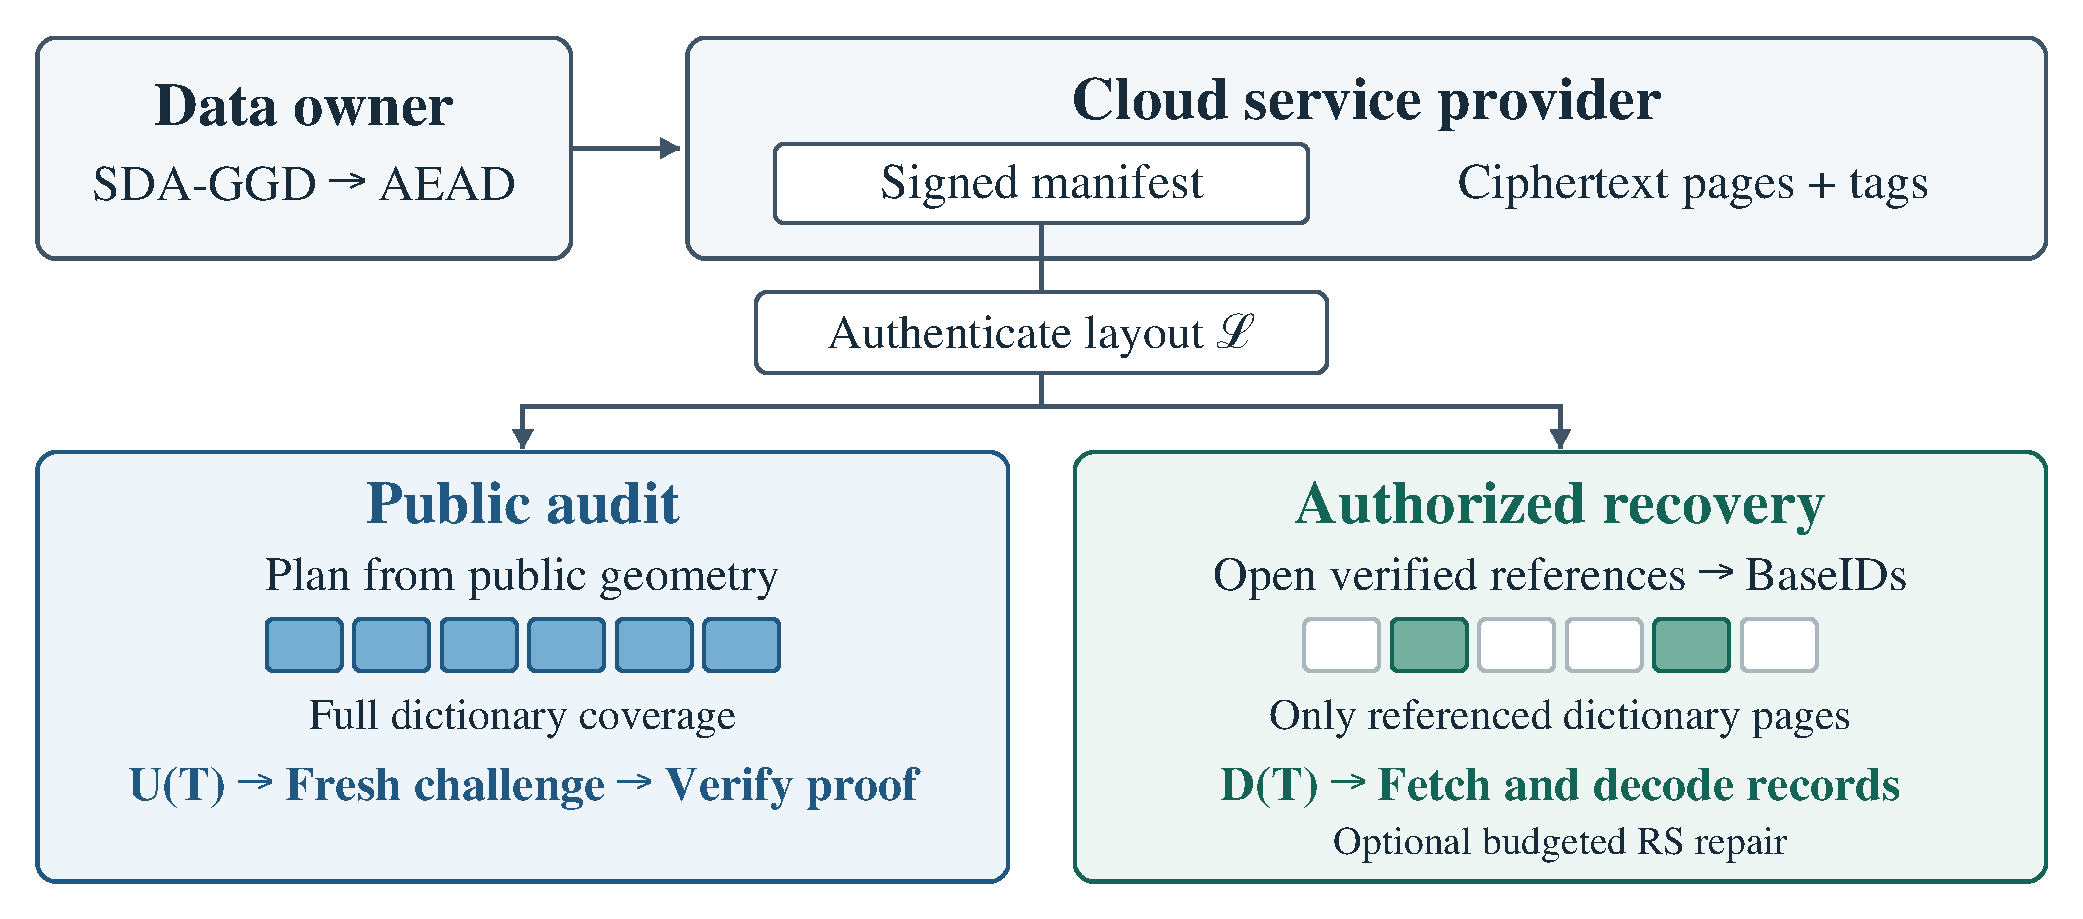
\includegraphics[width=\textwidth]{figures/architecture.pdf}
\caption{ARC-Audit system architecture. The page strips illustrate dictionary coverage for public auditing and authorized recovery.}
\label{fig:architecture}\end{figure*}

\section{ARC-Audit Design}\label{sec:design}
\subsection{Overview}
Fig.~\ref{fig:architecture} illustrates how public auditing and authorized recovery derive distinct page sets from the same encoded batch. The owner encodes records with SDA-GGD, seals the resulting logical container into addressable ciphertext pages, and commits to their layout in a signed manifest, which both clients authenticate against their provisioned pins. To audit target records $T$, the public verifier includes all dictionary pages of the relevant groups in each record's sufficient closure and merges overlapping closures into $U(T)$ before issuing a fresh aggregate challenge. To recover records, the authorized retriever first authenticates and decrypts the reference pages to extract BaseIDs, resolves the exact dependency set $D(T)$ from the referenced dictionary rows, retrieves the remaining pages, and decodes the canonical records only after all required inputs pass verification.

To tolerate page losses within a storage budget, a protection layer deploys erasure-coding redundancy over selected ciphertext objects and serves repaired pages through the same authenticated verification path.

\subsection{Cost-Confirmed Shared Representation}\label{sec:c1}
SDA-GGD merges correlated fields to reduce encoded size while preserving the span boundaries required for page-level dependency planning. Candidate merges are ranked by sampled byte gains and committed only if confirmed by the full-input serialized cost. The resulting public layout records stream spans and dictionary ranges so that a verifier can resolve audit pages without inspecting encrypted references.

\emph{Encoding and serialized cost.}
Under the declared schema, each field is assigned an exact decimal scale and integer width. Constant fields are stored once, while nonconstant fields are partitioned into groups. For a group $G$ of total bit width $L_g$, the encoder selects $k$ base-bit positions covering $M_g$ distinct observed bases and leaves the remaining $L_g-k$ positions as the per-record deviation. Each record stores a fixed-width base identifier of $b_g=\lceil\log_2 M_g\rceil$ bits alongside its deviation, while the group dictionary stores the unique bases.

For $n$ records, the serialized group cost is
\begin{equation}\label{eq:cost}
\begin{split}
C(G)={}&C_{\mathrm{hdr}}(G,k)+\lceil M_gk/8\rceil+\lceil nb_g/8\rceil\\
 &+\lceil n(L_g-k)/8\rceil,
\end{split}
\end{equation}
where $C_{\mathrm{hdr}}(G,k)=11+2|G|+2k$ bytes encodes the group mode, field identifiers, and base-bit positions, and a RAW group costs $C_{\mathrm{hdr}}(G,0)+\lceil nL_g/8\rceil$. Because streams are serialized separately, each term is byte-rounded independently. The total logical container cost is $C_0+\sum_G C(G)$, where $C_0$ accounts for the fixed schema, constants, timestamp/label representation, and global header.

\emph{Within-group configuration.}
$\operatorname{Config}(X,G)$ stably orders the local bit positions of $G$ by nondecreasing empirical binary entropy (preserving concatenation order on ties within merged groups) and evaluates prefixes of length $k=0,1,\ldots,L_g$, halting once $M_g=n$. Letting $n_v$ count the records sharing base $v$, a prefix is feasible under a configured dependency cap $\rho\in(0,1]$ if $R_{\mathrm{dep}}=\max_v n_v/n\leq\rho$. The configurator selects the feasible prefix minimizing the serialized cost in Eq.~\eqref{eq:cost} (breaking ties by smaller $k$), or, if no prefix is feasible, minimizes $R_{\mathrm{dep}}$ followed by cost and smaller $k$. It falls back to RAW whenever the RAW cost does not exceed that of the selected GD configuration.

\emph{Sample ranking and full-data confirmation.}
Grouping initializes each nonconstant field as a singleton active group and evaluates candidate merges over a fixed sample using the joint byte gain $\widehat\Delta=C_m(G_a)+C_m(G_b)-C_m(G_a\mathbin{\|}G_b)$, where $C_m$ configures and measures each group on the sampled rows and $\|$ denotes ordered field concatenation. Pairs with positive sampled gain enter a priority queue. Prior to full-input confirmation, candidates are refreshed against the current sample state and obsolete versions are discarded. Before committing a merge between $G_a$ and $G_b$, the encoder reconfigures $G_a\mathbin{\|}G_b$ over all input records and computes
\begin{equation}
\Delta_{\mathrm{full}}=C(G_a)+C(G_b)-C(G_a\mathbin{\|}G_b).
\end{equation}
A merge is accepted only when both the full-input serialized-byte gain and payload gain are strictly positive, after which affected candidates are updated until the queue empties (with RAW fallback reflected in each configuration's byte cost). Algorithm~\ref{alg:grouping} formalizes this procedure over exact records $X$, schema $\Sigma$, and sample indices $I$: $\operatorname{Config}(X,G)$ returns the optimal group configuration including RAW fallback, $C(G;c)$ and $C_{\mathrm{pay}}(G;c)$ denote the serialized cost and header-excluded payload cost under configuration $c$ (omitting $c$ refers to the active configuration), and $\operatorname{SampleGain}$ returns the sampled gain and configuration without authorizing a merge on its own.

Because merging two groups can alter the gains of adjacent pairs, Algorithm~\ref{alg:grouping} records rejected versioned pairs in $J$ and discards stale entries whose endpoint versions have changed. To prevent candidates whose refreshed gain decreases from stalling the queue or looping indefinitely, $\operatorname{TopGain}$ reports the current queue-head gain ($-\infty$ if empty), ties follow insertion order, and each candidate may be deferred at most $d_{\max}=8$ times (tracked by $d_e$) before full-input examination.

\begin{algorithm}[t]\centering\normalsize\setcounter{algline}{0}
\caption{Cost-Confirmed Grouping.}\label{alg:grouping}
\begin{tabular}{@{}r@{\enspace} >{\raggedright\arraybackslash}p{.88\columnwidth}@{}}
\multicolumn{2}{@{}p{\columnwidth}@{}}{\textbf{Require:} Records $X$, schema $\Sigma$, sample indices $I$.}\\
\multicolumn{2}{@{}p{\columnwidth}@{}}{\textbf{Ensure:} Logical container $F$ and public layout $\mathcal L$.}\\
\al & $\mathcal G\gets$ singleton nonconstant-field groups.\\
\al & Configure $\mathcal G$ on $X$ and $X_I$; $J\gets\varnothing$.\\
\al & $Q\gets$ positive sampled-gain pairs; initialize $d_e=0$.\\
\al & \textbf{while} $Q\neq\varnothing$ \textbf{do}\\
\al & \hspace*{1em}$e=(G_a,G_b,\text{versions})\gets\operatorname{PopMax}(Q)$.\\
\al & \hspace*{1em}\textbf{if} $e$ is stale or $e\in J$, \textbf{continue}.\\
\al & \hspace*{1em}$(\widehat\Delta,\widehat c)\gets\operatorname{SampleGain}(X_I,G_a,G_b)$.\\
\al & \hspace*{1em}\textbf{if} $\widehat\Delta\leq0$, add $e$ to $J$; \textbf{continue}.\\
\al & \hspace*{1em}\textbf{if} $\operatorname{TopGain}(Q)>\widehat\Delta$ and $d_e<d_{\max}$ \textbf{then}\\
\al & \hspace*{2em}$d_e\gets d_e+1$; requeue $e$ with $\widehat\Delta$; \textbf{continue}.\\
\al & \hspace*{1em}\textbf{end if}\\
\al & \hspace*{1em}$G_c\gets G_a\mathbin{\|}G_b$; $c\gets\operatorname{Config}(X,G_c)$.\\
\al & \hspace*{1em}$\Delta_{\mathrm{full}}\gets C(G_a)+C(G_b)-C(G_c;c)$.\\
\al & \hspace*{1em}$\Delta_P\gets C_{\mathrm{pay}}(G_a)+C_{\mathrm{pay}}(G_b)-C_{\mathrm{pay}}(G_c;c)$.\\
\al & \hspace*{1em}\textbf{if} $\Delta_{\mathrm{full}}>0$ and $\Delta_P>0$ \textbf{then}\\
\al & \hspace*{2em}Replace $G_a,G_b$ in $\mathcal G$ by $G_c$ with $(c,\widehat c)$.\\
\al & \hspace*{2em}Invalidate old-group entries; queue positive new/live pairs.\\
\al & \hspace*{1em}\textbf{else} add $e$ to $J$.\\
\al & \hspace*{1em}\textbf{end if}\\
\al & \textbf{end while}\\
\al & $(F,\mathcal L)\gets\operatorname{Serialize}(X,\Sigma,\mathcal G)$.\\
\al & \textbf{return} $(F,\mathcal L)$.\\\bottomrule
\end{tabular}
\end{algorithm}

\begin{proposition}{Confirmed logical cost reduction}\label{prop:cost}
Every accepted merge strictly decreases both the checked logical serialized
cost and its payload cost. Starting from $g_0$ active groups, at most
$g_0-1$ merges are accepted.
\end{proposition}
\begin{claimproof}
Algorithm~\ref{alg:grouping} accepts a merge only if both the full-input serialized gain and the payload gain are positive. Since the costs of other groups and the fixed container component stay unchanged, each merge strictly reduces both costs. Each merge also reduces the number of active groups by one, so the algorithm accepts at most $g_0-1$ merges. Recording rejected versioned pairs, discarding obsolete entries, and limiting requeues ensure that candidate processing terminates between merges.
\end{claimproof}
The measured secure cloud cost in Eq.~\eqref{eq:cloud-cost} additionally includes encryption framing, audit tags, and the public manifest. Section~\ref{sec:eval} evaluates that final cost separately from the logical grouping objective.


\subsection{Page Encryption and Authenticated Layout}\label{sec:seal}
ARC-Audit uses page encryption and an authenticated layout to separate the structural information needed to locate dependencies from the values needed to decode them. The public layout contains stream positions, widths, modes, base-bit positions, dictionary cardinalities, and record counts. This geometry supports the page mapping in Eq.~\eqref{eq:phi}, while the private decoding header and values, including numeric constants and private field values, remain in the encrypted slices of the complete logical container together with the encoded records.

For each construction, the owner samples a fresh 256-bit batch identifier
$b$ and a random encryption master secret, then derives $k_b$ via HKDF-SHA256 with
salt $b$ and context \texttt{ARC/ENC/v1}~\cite{RFC5869}.
Each slice uses the 96-bit encoding of its local page index as the nonce $N_p$, so page nonces are distinct under $k_b$. The associated data $A_p$ canonically encodes the protocol, owner domain, batch, object identity, codec, and plaintext length, and these fields are retained in the public descriptor. With $P_0=4{,}068$ B, AES-256-GCM seals each slice as~\cite{RFC5116}
\begin{equation}\label{eq:cipher}
C_p=N_p\,\|\,\mathsf{Enc}_{k_b}(N_p,F_p,A_p).
\end{equation}
The 12-byte nonce and 16-byte authentication tag give a valid ciphertext length of $\ell(p)=|F_p|+28\leq4{,}096$ B, while the final slice retains its actual length. A container of $B_F>0$ bytes has $N=\lceil B_F/P_0\rceil$ pages and occupies $B_{\rm cipher}=B_F+28N$ ciphertext bytes, as virtual zeros used for auditing and repair add no stored ciphertext bytes.

Each descriptor also records the complete ciphertext length and SHA-256 digest, and the corresponding audit tag binds this descriptor to the public-parameter fingerprint. After generating all ciphertext objects and tags, the owner serializes the tags in ascending page-index order and signs a canonical manifest containing the object descriptors, public layout, audit parameters, and SHA-256 digest of the tag file using Ed25519. The resulting 32-byte manifest digest and 32-byte signing public key serve as the clients' provisioned pins. This ordering binds tags to immutable ciphertexts and binds the manifest to completed tags without introducing a circular digest dependency (Algorithm~\ref{alg:seal}).

\begin{algorithm}[t]\centering\normalsize\setcounter{algline}{0}
\caption{Seal a Data Batch.}\label{alg:seal}
\begin{tabular}{@{}r@{\enspace} >{\raggedright\arraybackslash}p{.88\columnwidth}@{}}
\multicolumn{2}{@{}p{\columnwidth}@{}}{\textbf{Require:} Logical container $F$, public layout $\mathcal L$, owner domain.}\\
\multicolumn{2}{@{}p{\columnwidth}@{}}{\textbf{Ensure:} Ciphertext objects, audit tags, signed manifest, and client pins.}\\
\al & Sample fresh batch $b$ and encryption master secret; derive $k_b$.\\
\al & Generate independent audit secret $x$, public parameters $\mathsf{pp}$, and a manifest signing key.\\
\al & \textbf{for each} slice $F_p$ of at most 4,068 B \textbf{do}\\
\al & \hspace*{1em}$N_p\gets\operatorname{Encode}_{96}(p)$; form associated data $A_p$.\\
\al & \hspace*{1em}$C_p\gets N_p\|\mathsf{Enc}_{k_b}(N_p,F_p,A_p)$.\\
\al & \hspace*{1em}$d_p\gets(A_p,|C_p|,\mathsf{SHA256}(C_p))$.\\
\al & \hspace*{1em}$\tau_p\gets\operatorname{Tag}(x,\mathsf{pp},d_p,C_p)$.\\
\al & \textbf{end for}\\
\al & Serialize tags in page-index order to obtain $B_\tau$.\\
\al & $M\gets\operatorname{Manifest}(b,\mathcal L,\{d_p\},\mathsf{pp},\mathsf{SHA256}(B_\tau))$.\\
\al & Sign canonical $M$; provision signing public key and $\mathsf{SHA256}(M)$ as pins.\\
\al & Retain batch-scoped private encoding state and decryption capability.\\
\al & \textbf{return} $\{C_p\},\{\tau_p\},M$, signature, and pins.\\\bottomrule
\end{tabular}\end{algorithm}

\subsection{Authenticated Recovery Closure}\label{sec:c2}
Given a target set $T$ and authenticated layout $\mathcal L$, public closure planning computes the sufficient page union $U(T)$ directly from public geometry by including the full dictionary of each relevant group. Under the bit-span map $\Phi_{\mathcal L}$, let $S$ denote the pages covering private structural metadata, $R_g(i)$ and $V_g(i)$ the pages covering record $i$'s reference and deviation (or RAW) spans in group $g$, $L(i)$ the pages covering its labels, and $\mathcal P_g^{\rm dict}$ all mapped dictionary pages for a GD group. The single-record public recovery closure is
\begin{equation}\label{eq:closure}
K(i)=S\cup L(i)\cup\bigcup_g
\bigl(R_g(i)\cup V_g(i)\cup\mathcal P_g^{\rm dict}\bigr),
\end{equation}
where $R_g(i)$ and $\mathcal P_g^{\rm dict}$ are empty for RAW groups. Because $\Phi_{\mathcal L}$ captures every page intersecting a selected span, a page shared across multiple logical streams is included whenever any target span intersects it.

While the public verifier forms $K(i)$ from $\mathcal L$ to cover every row selectable by a valid BaseID, the authorized retriever authenticates and decrypts $S$ and the reference pages, extracts and range-checks each BaseID at its committed offset, and maps only the referenced dictionary rows. Combining those dictionary-row pages with $S$, references, local content, and labels yields the exact dependency set $\mathcal D(i)$.

Across a multi-record request $T$, public planning merges overlapping per-record closures into $U(T)=\bigcup_{i\in T}K(i)$. Given ciphertext lengths $\ell(p)$, the logical bytes read under union planning and uncached per-record traversal are
\begin{equation}\label{eq:reads}
B_U=\sum_{p\in U(T)}\ell(p),\qquad
B_N=\sum_{i\in T}\sum_{p\in K(i)}\ell(p).
\end{equation}
Request-local caching can likewise avoid duplicate object reads during per-record traversal, so our experimental controls separate read reuse (via caching or union planning) from proof aggregation. For cross-batch requests, the verifier computes target sets and page unions per batch and aggregates them using batch-qualified object identifiers.

\subsection{Fresh Public Aggregate Audit}\label{sec:audit}
The public aggregate interface (Public-Aggregate) verifies a linear homomorphic response over the public closure $U$, binding the target set, snapshot, and selected pages to a fresh challenge so that responses cannot be replayed across requests or versions.

Each complete ciphertext object is partitioned into $s=133$ little-endian sectors of 31 B, with virtual zero padding beyond its valid length. Each sector integer satisfies $m_{p,j}<2^{248}<q$ for the BLS12-381 scalar order $q$, ensuring that sectorization spans the nonce, encrypted payload, and AEAD tag while the signed valid length governs tail truncation.

Following the Shacham--Waters linear public authenticator~\cite{ShachamWaters2013}, the owner samples a secret key $x$, publishes $Y=xg_2$, and computes tags in $\mathbb G_1$ under a pairing $e:\mathbb G_1\times\mathbb G_2\to\mathbb G_T$ as
\begin{equation}\label{eq:tag}
\tau_p=x\left(H(W_p)+\sum_{j=1}^{s}m_{p,j}u_j\right),
\end{equation}
where $W_p$ binds the complete ciphertext descriptor and parameter fingerprint, and both the sector bases $u_j$ and descriptor hash $H$ are instantiated with domain-separated hash-to-curve mappings~\cite{RFC9380}.

For each batch request, the verifier draws a fresh 256-bit nonce and forms a canonical challenge binding the snapshot, public parameters, target set, selected page set, request policy, and session. Challenge coefficients $\nu_p\in\mathbb F_q^*$ are deterministically expanded via SHA-512 over the canonical-challenge digest, page index, and a retry counter, reducing outputs modulo $q$ and incrementing the counter on zero. Upon receiving the challenge, the CSP reads each selected page once and returns
\begin{equation}\label{eq:aggregate}
\sigma=\sum_{p\in U}\nu_p\tau_p,\qquad
\mu_j=\sum_{p\in U}\nu_pm_{p,j}\pmod q.
\end{equation}
After verifying challenge context, framing, point and subgroup membership, scalar bounds, and vector dimensions against its own expected page set (excluding invalid or identity bases in the public parameters), the verifier checks the pairing equation
\begin{equation}\label{eq:pairing}
e(\sigma,g_2)=e\left(\sum_{p\in U}\nu_pH(W_p)+\sum_j\mu_ju_j,Y\right).
\end{equation}
Algorithm~\ref{alg:audit} summarizes the public audit protocol.

\begin{algorithm}[t]\centering\normalsize\setcounter{algline}{0}
\caption{ARC-Audit Public Closure Audit.}\label{alg:audit}
\begin{tabular}{@{}r@{\enspace} >{\raggedright\arraybackslash}p{.88\columnwidth}@{}}
\multicolumn{2}{@{}p{\columnwidth}@{}}{\textbf{Require:} Targets $T$, corresponding manifests and pins, public audit parameters.}\\
\multicolumn{2}{@{}p{\columnwidth}@{}}{\textbf{Ensure:} \texttt{ACCEPT} or \texttt{REJECT}.}\\
\al & \textbf{if} $T=\varnothing$, \textbf{return} \texttt{REJECT}. Partition $T$ into per-batch sets $\{T_b\}$.\\
\al & \textbf{for each} involved batch $b$ \textbf{do}\\
\al & \hspace*{1em}Authenticate its manifest against the pins. Check target ranges, uniqueness, and public parameters.\\
\al & \hspace*{1em}\textbf{if} validation fails, \textbf{return} \texttt{REJECT}.\\
\al & \hspace*{1em}$U_b\gets\operatorname{SortUnique}(\bigcup_{i\in T_b}K_{\mathcal L_b}(i))$.\\
\al & \hspace*{1em}Sample fresh nonce; bind expected snapshot, request, $T_b$, and $U_b$.\\
\al & \hspace*{1em}Derive $\nu_p\in\mathbb F_q^*$ for $p\in U_b$; send challenge and retain expected context.\\
\al & \hspace*{1em}CSP reads unique $C_p$ and uses $\tau_p$ for $p\in U_b$ to respond by Eq.~\eqref{eq:aggregate}.\\
\al & \hspace*{1em}Verifier checks framing, context, encodings, and Eq.~\eqref{eq:pairing}.\\
\al & \hspace*{1em}\textbf{if} the response is missing or any check fails, \textbf{return} \texttt{REJECT}.\\
\al & \textbf{end for}\\
\al & \textbf{return} \texttt{ACCEPT}.\\\bottomrule
\end{tabular}\end{algorithm}

The serialized aggregate proof occupies $4+2+48+133\cdot32=4{,}310$ B per batch, accounting for framing, the sector count, the aggregate point, and the scalar vector. A request involving $b_T$ batches therefore has $4{,}310 b_T$ proof bytes, in addition to declarations and challenges. Section~\ref{sec:eval} compares
this public interface with authorized reference discovery and public download
using their actual application framing.

For a fixed challenge, the individual-proof control returns
$(\nu_p\tau_p,(\nu_pm_{p,j})_j)$ for each $p$ and verifies the corresponding
single-page equation. Aggregate and individual responses therefore use the
same selected pages and fresh coefficients. Each individual proof adds an
8-byte page identifier to the 4,310 B proof format, so its total for $u$ pages
is $4{,}318u$ B.

\subsection{Authenticated Exact Record Recovery}\label{sec:c3}
ARC-Audit's exact recovery policy (Exact) authenticates and parses references before fetching the remaining record dependencies. The retriever begins by validating the manifest, version pins, and any sidecar binding. In Stage 1, it fetches the structural and reference ciphertext pages, checks each object's identity, length, and committed digest, and performs AEAD decryption. Only after authenticating those plaintexts does it parse the private structure and BaseIDs, validate their ranges, and resolve the exact dependency set $D(T)$. In Stage 2, it retrieves the remaining pages covering referenced dictionary rows, deviations, RAW content, and target labels through the same verified path.

A request-local cache retains verified ciphertexts and authenticated plaintexts so that pages fetched during reference discovery are reused in Stage 2. Before decoding, the retriever validates private decoder framing against the authenticated public layout and verifies that every bit span read lies within authenticated plaintext, returning $\bot$ on any authentication, range, framing, or decoding failure. Algorithm~\ref{alg:recovery} details single-batch recovery, and multi-batch requests execute the same procedure per involved batch.

Specifically, the helper $\operatorname{VerifiedOpen}$ retrieves the committed ciphertext for a requested page either directly or via the protected repair interface, verifies its descriptor, performs AEAD decryption, and returns either the authenticated plaintext (caching only verified ciphertext and plaintext) or $\bot$.

\begin{algorithm}[t]\centering\normalsize\setcounter{algline}{0}
\caption{Authenticated Exact Record Recovery.}\label{alg:recovery}
\begin{tabular}{@{}r@{\enspace} >{\raggedright\arraybackslash}p{.88\columnwidth}@{}}
\multicolumn{2}{@{}p{\columnwidth}@{}}{\textbf{Require:} Manifest and pins, decryption capability, targets $T$, cloud fetch interface, and optionally a signed sidecar with its provisioned public key and digest.}\\
\multicolumn{2}{@{}p{\columnwidth}@{}}{\textbf{Ensure:} Complete decoded records $\{\widehat r_i\}_{i\in T}$ or $\bot$.}\\
\al & Authenticate the manifest and validate $T$. If present, authenticate the sidecar against its own pin and check its binding to the batch snapshot.\\
\al & \textbf{if} validation fails, \textbf{return} $\bot$.\\
\al & $D_0(T)\gets S\cup\bigcup_{i\in T,g}R_g(i)$; $\mathcal C\gets\varnothing$.\\
\al & \textbf{for each} $p\in D_0(T)$ \textbf{do}\\
\al & \hspace*{1em}$\mathcal C[p]\gets\operatorname{VerifiedOpen}(p)$; on failure \textbf{return} $\bot$.\\
\al & \textbf{end for}\\
\al & Parse the authenticated private structure and BaseIDs.\\
\al & \textbf{if} parsing fails or any BaseID is out of range, \textbf{return} $\bot$.\\
\al & Form $D(T)$ by adding to $D_0(T)$ the pages covering target deviations or RAW data, labels, and the dictionary rows selected by the validated BaseIDs.\\
\al & \textbf{for each} $p\in D(T)\setminus\operatorname{dom}(\mathcal C)$ \textbf{do}\\
\al & \hspace*{1em}$\mathcal C[p]\gets\operatorname{VerifiedOpen}(p)$; on failure \textbf{return} $\bot$.\\
\al & \textbf{end for}\\
\al & Check private/public framing and decode from $\mathcal C$.\\
\al & \textbf{if} framing or complete decoding fails, \textbf{return} $\bot$.\\
\al & \textbf{return} $\{\widehat r_i\}_{i\in T}$.\\\bottomrule
\end{tabular}\end{algorithm}

The Conservative control
replaces $D_0(T)$ in line 3 with $U(T)$, while subsequent authentication and decoding remain
identical. Exact recovery can thus proceed when an unused dictionary object
is unavailable, provided its actual decoding inputs are available or repairable.

\subsection{Budgeted Ciphertext Protection}\label{sec:protection}
Because a shared page can support multiple records, choosing which pages to protect governs record survivability under a fixed storage cap. ARC-Audit applies systematic erasure coding to prioritized ciphertext objects and subjects repaired pages to full integrity verification prior to decoding.

A systematic RS$(10,8)$ sidecar over GF$(256)$ organizes eight ciphertext objects per stripe and stores two parity shards per stripe while leaving original ciphertexts in place. Objects shorter than 4,096 B are virtually zero-padded during encoding, and incomplete stripes use declared virtual zero slots. Parity is computed over the complete ciphertext including the nonce and AEAD tag, and a signed sidecar manifest binds the parent snapshot, code parameters, stripe membership, and parity digests.

Under a fractional storage budget $\beta$, we evaluate three protection rankings: Dictionary prioritizes dictionary-bearing pages ahead of other objects, Uniform applies a seeded permutation, and FrequencyD ranks objects by their dependency frequency across a reference record set. All three policies share a common stripe count chosen so that every serialized sidecar satisfies the per-batch cap
\begin{equation}\label{eq:budget}
B_{\rm side,b}\leq\left\lfloor\beta B_{\rm cipher,b}\right\rfloor.
\end{equation}
Each admitted stripe stores two 4,096-byte parity shards, giving a total charge of $8{,}192s_R+|M_R|+128$ bytes for $s_R$ stripes and serialized sidecar manifest $M_R$, where the final 128 bytes account for the signature, signing public key, and digest pin. Stripe admission is governed by the largest charge among the three rankings. Our evaluation sets $\beta=0.10$ and includes NoEC as a zero-redundancy baseline.

During protected retrieval, if an original ciphertext object is unavailable, the retriever authenticates the available original and parity shards in its stripe against their committed digests and counts the declared virtual zero slots. Once eight distinct valid slots are available in the stripe, RS decoding reconstructs the missing object, truncates it to its committed ciphertext length, and verifies its original ciphertext digest before caching and AEAD decryption. The same repair helper serves both reference discovery and exact dependency acquisition.

\subsection{Computation and Storage Accounting}\label{sec:accounting}
Let $N$ denote the number of ciphertext objects in a batch and $u=|U(T)|$. Beyond resident authenticated metadata, direct closure enumeration incurs expected $O(\sum_{i\in T}|K(i)|)$ set-insertion work and $O(u)$ unique-object state, while grouping cost aggregates all sampled configurations, full-input reconfigurations, and queue updates actually executed (with each accepted merge reducing the active-group count by one).

Audit tag generation processes $Ns$ sectors. For proof generation, the CSP accumulates $us$ field multiplications and $u$ weighted tags, whereas the verifier computes $u$ descriptor-hash terms and $s$ sector-base terms followed by two pairings. Multi-batch request costs sum across involved batches: proof size stays fixed per batch, challenge material scales with the selected page set, and the manifest scales with $N$.

Without a protection sidecar, secure cloud storage is
\begin{equation}\label{eq:cloud-cost}
B_{\rm cloud}=B_{\rm cipher}+B_{\rm tags}+B_{\rm manifest},
\end{equation}
where $B_{\rm tags}=48N$ bytes and the signed manifest embeds the public parameters, while AEAD overhead contributes $28N$ bytes to $B_{\rm cipher}$. Owner-side base bytes and total private state are tracked separately. Deploying a protection sidecar adds its cloud files and provisioned client pins, keeping cloud storage distinct from client state.

Application-layer traffic accounts for declarations, challenges, responses, and any first-stage reference material required by the interface, with each ciphertext page message adding an 8-byte framing-and-count prefix and a 12-byte per-page identifier-and-length header. Request timers start after batch context initialization completes manifest and parameter verification, and recovery timing encompasses retrieval or repair, verification, decryption, and decoding. Because reconstructing one missing page may require fetching multiple stripe shards, server-side reads are reported separately from application-layer reply bytes.

\section{Security and Recoverability Analysis}\label{sec:security}
We now analyze the correctness and security guarantees of ARC-Audit under the system model of Section~\ref{sec:model}. We begin by establishing decoding correctness and closure coverage, then bound returned-record authenticity, equal-leakage content confidentiality, and aggregate audit response authenticity, and conclude with sufficient conditions for recovery under erasures. Let $C_p$ and $F_p$ denote the original ciphertext and corresponding plaintext slice of page $p$ in the expected snapshot.

\subsection{Representation Correctness and Closure Coverage}\label{sec:representation-proof}\label{sec:closure-proof}
\begin{proposition}{Correct decoding and closure coverage}\label{prop:representation}\label{prop:closure}
For a correctly constructed batch, the original dependency pages suffice to decode the target records. For every valid target set $T$, $D(T)\subseteq U(T)$.
\end{proposition}
\begin{claimproof}
Let $x_{i,g}$ be the bit string of record $i$ in GD group $g$, with base-bit positions $I_g$ and complementary deviation positions $J_g$. By construction, the encoder enforces
\begin{equation}
x_{i,g}[I_g]=B_{g,\mathrm{ID}_{i,g}},\qquad
x_{i,g}[J_g]=d_{i,g}.
\end{equation}
The decoder reassembles $x_{i,g}$ by placing the dictionary row and deviation into $I_g$ and $J_g$, inverts field widths and exact decimal scaling, and decodes RAW, constant, timestamp, and label fields under the declared schema to recover the canonical record $r_i$.

Let $L_{g,\mathrm{ID}_{i,g}}$ denote the logical bit interval of the referenced dictionary row and $L_g^{\mathrm{dict}}$ the full dictionary interval of group $g$. Because $\Phi_{\mathcal L}$ returns all pages intersecting an interval,
\begin{equation}
L_{g,\mathrm{ID}_{i,g}}\subseteq L_g^{\mathrm{dict}}
\ \Longrightarrow\
\Phi_{\mathcal L}(L_{g,\mathrm{ID}_{i,g}})
\subseteq\Phi_{\mathcal L}(L_g^{\mathrm{dict}}).
\end{equation}
Since both policies cover structural metadata, references, local data, and labels, taking unions over groups and targets yields
\begin{equation}
\mathcal D_{\mathcal L}(i)\subseteq K_{\mathcal L}(i)
\ \Longrightarrow\ D(T)\subseteq U(T).
\end{equation}
\end{claimproof}

\subsection{Authenticated Binding and Returned-Record Authenticity}\label{sec:binding}\label{sec:conditional}
Let $\mathsf{BadSig}$ denote the event that a canonical message never signed by the owner passes signature verification under the trusted public key, and let $\mathsf{BadDig}$ denote the event that an accepted manifest, page, or digest-bound protection object differs in bytes from the object originally committed under that digest. The verifier pins the primary manifest by its trusted digest, verifies sidecar binding to the parent snapshot, and checks any deployment-specified protection layout identity.

\begin{proposition}{Returned-record authenticity}\label{prop:record-auth}
Let $\mathsf{WrongRec}$ denote successful recovery with at least one record differing from its canonical value in the expected snapshot. For every probabilistic polynomial-time adversary there are reductions $\mathcal B_{\rm sig}$ and $\mathcal B_{\rm dig}$ such that
\begin{equation}\label{eq:record-auth}
\begin{aligned}
\Pr[\mathsf{WrongRec}]
&\leq \Pr[\mathsf{BadSig}]+\Pr[\mathsf{BadDig}]\\
&\leq \operatorname{Adv}^{\rm EUF\text{-}CMA}_{\rm Sig}(\mathcal B_{\rm sig})
+\operatorname{Adv}^{\rm CR}_{H_{\rm dig}}(\mathcal B_{\rm dig}).
\end{aligned}
\end{equation}
\end{proposition}
\begin{claimproof}
Define $\mathsf{Good}=\neg(\mathsf{BadSig}\lor\mathsf{BadDig})$. Every candidate page $C'_p$ obtained via direct retrieval or RS repair must pass identity, length, context, and committed manifest-digest checks. Conditioned on $\mathsf{Good}$,
\begin{equation}
\begin{aligned}
H_{\rm dig}(C'_p)=H_{\rm dig}(C_p)&\ \Longrightarrow\ C'_p=C_p\\
&\ \Longrightarrow\ \operatorname{Open}_{k_b,N_p,A_p}(C'_p)=F_p.
\end{aligned}
\end{equation}
Hence, Stage 1 opens the authentic reference pages and derives $\widehat D(T)=D(T)$ from verified BaseIDs, while Stage 2 enforces the identical acceptance rule on the remaining dependency pages. By Proposition~\ref{prop:representation},
\begin{equation}
\begin{aligned}
\mathsf{Good}\land\mathsf{RecAccept}&\ \Longrightarrow\ \widehat{\mathbf r}_T=\mathbf r_T,\\
\widehat{\mathbf r}_T&=\operatorname{Decode}_T\bigl((F_p)_{p\in D(T)}\bigr).
\end{aligned}
\end{equation}
Consequently, $\mathsf{WrongRec}\subseteq\mathsf{BadSig}\cup\mathsf{BadDig}$. Extracting the first newly accepted forged message-signature pair yields $\mathcal B_{\rm sig}$, extracting the first colliding pair of distinct accepted objects yields $\mathcal B_{\rm dig}$, and a union bound establishes Eq.~\eqref{eq:record-auth}. In multi-owner deployments, the bound sums over the relevant signing keys.
\end{claimproof}

\subsection{Content Confidentiality under the Public View}\label{sec:confidentiality}
In the confidentiality game, the adversary chooses canonical inputs $X_0,X_1$ satisfying $\mathsf{Leak}(X_0)=\mathsf{Leak}(X_1)$, where for fixed public construction parameters $\mathsf{Leak}$ captures page counts and lengths, associated data, public layout, dictionary cardinalities, and visible protection layouts. The challenger seals one randomly selected input, publishes the public storage state, and answers adaptive public audit queries, with the adversary's advantage defined as the absolute difference in its probabilities of outputting $1$ across the two branches. Whenever a deployment exposes authorized recovery access traces induced by private BaseIDs, those traces enter its leakage profile.

\begin{proposition}{Content confidentiality under equal leakage}\label{prop:confidentiality}
If the derived batch keys are indistinguishable from independent random keys and AEAD provides nonce-respecting multi-message confidentiality, then for every probabilistic polynomial-time public observer $\mathcal A$,
\begin{equation}
\operatorname{Adv}^{\rm priv}_{\rm ARC}(\mathcal A)
\leq 2\varepsilon_{\rm KDF}+\sum_{b=1}^{B}\varepsilon_{{\rm AEAD},b}.
\end{equation}
Here $\varepsilon_{\rm KDF}$ bounds the advantage of replacing all $B$ batch keys in one input branch, and $\varepsilon_{{\rm AEAD},b}$ bounds multi-message distinguishing advantage for batch $b$.
\end{proposition}
\begin{claimproof}
Let $\mathsf{Real}(X)$ use KDF-derived keys and $\mathsf{Rand}(X)$ substitute independent random keys across the hybrid sequence
\begin{equation}
\begin{aligned}
\mathsf{Real}(X_0)
&\xrightarrow{\rm KDF}\mathsf{Rand}(X_0)\\
&\xrightarrow{{\rm AEAD},\,b=1,\ldots,B}\mathsf{Rand}(X_1)
\xrightarrow{\rm KDF}\mathsf{Real}(X_1).
\end{aligned}
\end{equation}
Each batch transition encrypts equal-length plaintext pairs under identical associated data, with distinct nonces derived from local page indices under each batch key. Given the challenge ciphertexts and public layout, the simulator generates independent signing and audit keys to compute digests, tags, signatures, and RS parity shards directly from the ciphertexts. Because public audit page sets depend solely on the public layout and request policy, the simulator answers all adaptive audit queries consistently. Summing the distinguishing advantages across adjacent hybrids yields the stated bound.
\end{claimproof}

\subsection{Public Aggregate Audit Correctness and Response Authenticity}\label{sec:audit-scope}
The verifier derives $U$ from the authenticated layout and binds the expected snapshot, audit parameters, targets, selected pages, policy, session, and fresh nonce into a challenge context, from which it expands the coefficients $\nu_p$. Before pairing verification, the verifier validates response framing, dimensions, scalar bounds, curve points, and subgroup membership; the aggregate tag may represent the group identity and remains constrained by the pairing check.

\emph{Correctness.} Let $(\sigma^\star,\boldsymbol\mu^\star)$ denote the honest response. Substituting Eqs.~\eqref{eq:tag} and~\eqref{eq:aggregate} yields
\begin{equation}\label{eq:honest}
\begin{aligned}
\sigma^\star
&=\sum_{p\in U}\nu_p\tau_p\\
&=x\left(\sum_{p\in U}\nu_pH(W_p)+\sum_{j=1}^{s}\mu_j^\star u_j\right),\\
\mu_j^\star&=\sum_{p\in U}\nu_p m_{p,j}.
\end{aligned}
\end{equation}
Bilinearity and $Y=xg_2$ immediately imply Eq.~\eqref{eq:pairing}. Because each 31-byte sector encodes an integer strictly below $2^{248}<q$, the sector vector together with the signed valid length uniquely determines the ciphertext bytes.

\emph{Security experiment.} The owner honestly seals a batch and publishes its ciphertexts, tags, manifest, and public parameters. After interacting adaptively across multiple audit queries, the adversary wins if any challenged response satisfies
\begin{equation}\label{eq:bad-audit}
\mathsf{BadAudit}
=\{\mathsf{Verify}=1\land\boldsymbol\mu\ne\boldsymbol\mu^\star\}.
\end{equation}

\begin{proposition}{Selected-set response authenticity}\label{prop:audit}
Let $e$ be a prime-order Type-3 pairing, $x$ a uniformly random nonzero scalar, and $P$ a uniformly random nonidentity element of $\mathbb G_1$. Assume computing $xP$ from $(g_1,g_2,P,X_1=xg_1,X_2=xg_2)$ is hard. Model the basis derivation and descriptor hash as domain-separated random oracles. If the verifier uses the expected signed snapshot, the basis-derivation inputs are distinct, and descriptor-hash inputs uniquely bind committed pages, then $\Pr[\mathsf{BadAudit}]$ is negligible in the single-batch experiment.
\end{proposition}
\begin{claimproof}
The reduction embeds the challenge by setting $Y=X_2$, sampling independent $a_j,b_j,r_p\in\mathbb F_q$, and programming
\begin{equation}
\begin{aligned}
u_j &= a_jP+b_jg_1,\\
H(W_p)&=r_pg_1-\sum_{j=1}^{s}m_{p,j}u_j,\\
\tau_p&=r_pX_1,
\end{aligned}
\end{equation}
resampling $(a_j,b_j)$ if $u_j$ equals the identity. Uniform $b_j$ distributes each $u_j$ uniformly over $\mathbb G_1\setminus\{0\}$ while leaving $a_j$ uniform conditioned on $u_j$. Conditioned on the bases and page contents, independent $r_p$ ensure that distinct $H(W_p)$ outputs are independent and uniform. The reduction pre-programs these queries before publishing the batch and answers subsequent oracle queries consistently. By construction, the programmed tags satisfy Eq.~\eqref{eq:tag}, faithfully reproducing the real tag and response distribution.

For the first accepted incorrect response, let $\Delta_j=\mu_j-\mu_j^\star$. Dividing its pairing check by that of the honest response gives
\begin{equation}
e(\sigma-\sigma^\star,g_2)
=e\left(\sum_j\Delta_j u_j,X_2\right).
\end{equation}
By pairing nondegeneracy, $Q\mapsto e(Q,g_2)$ is injective on $\mathbb G_1$, whence
\begin{equation}
\begin{aligned}
\sigma-\sigma^\star&=x\sum_j\Delta_j u_j=\gamma\,xP+\eta X_1,\\
\gamma&=\sum_j\Delta_j a_j,\qquad \eta=\sum_j\Delta_j b_j.
\end{aligned}
\end{equation}
Because the adversary's view depends on the basis coins only through public $u_j$, the scalars $a_j$ remain independently uniform given the view, and $\boldsymbol\Delta\ne\mathbf 0$ implies $\Pr[\gamma=0]=1/q$. Whenever $\gamma\ne0$, the reduction recovers
\begin{equation}
xP=\gamma^{-1}(\sigma-\sigma^\star-\eta X_1).
\end{equation}
Thus, an adversary winning with probability $\varepsilon$ under genuine fixed metadata solves the assumed hard problem with probability at least $(1-1/q)\varepsilon$. Adding the metadata-binding failure probability yields the full single-batch bound, and independent per-batch audit keys enable a union bound across multi-batch responses.
\end{claimproof}
Proposition~\ref{prop:closure} guarantees that $U(T)$ covers all decoding dependencies, while Proposition~\ref{prop:audit} bounds the joint event that verification accepts an erroneous linear response over $U(T)$ under the deterministically expanded challenge coefficients. For multi-batch requests, acceptance with at least one erroneous batch response is bounded via a union bound over the involved batches. Record recovery additionally depends on whether the exact dependencies can be retrieved directly or reconstructed from repair shards.

\subsection{Conditional Recovery and Dependency Selection}\label{sec:recovery-condition}
Fix an authenticated protection layout and the object availability state during a request. Let $\mathcal A_0$ denote the set of directly available genuine original pages, $\mathcal P_{\rm prot}$ the protected pages, $S(p)$ the ten slots in the stripe containing $p$, and $\mathcal V$ the available authenticated slots including declared virtual zero slots. Define the effective recoverable page set as
\begin{equation}
\mathcal A_{\rm eff}=\mathcal A_0\cup
\bigl\{p\in\mathcal P_{\rm prot}:|S(p)\cap\mathcal V|\geq8\bigr\}.
\end{equation}
\begin{proposition}{Sufficient recovery condition}\label{prop:recovery}
If the metadata are authentic, the decryption keys are correct, and
\begin{equation}\label{eq:recovery-condition}
D(T)\subseteq\mathcal A_{\rm eff},
\end{equation}
then Exact recovery succeeds and returns the canonical records $\mathbf r_T$.
\end{proposition}
\begin{claimproof}
Let $G\in\mathbb F_{256}^{10\times8}$ be the systematic RS$(10,8)$ generator matrix. Selecting any eight distinct genuine slots $J$ within a stripe and letting $d_t$ hold the eight original symbols at byte offset $t$, the MDS property guarantees
\begin{equation}
c_{J,t}=G_Jd_t,\qquad\det G_J\ne0
\ \Longrightarrow\ d_t=G_J^{-1}c_{J,t}.
\end{equation}
Truncating the reconstructed object to its committed length yields the original ciphertext, which undergoes the same digest check and AEAD decryption as direct retrieval, making $F_p$ obtainable for every $p\in\mathcal A_{\rm eff}$.

Let $D_0(T)\subseteq D(T)$ be the pages required to parse structure and references. Condition~\eqref{eq:recovery-condition} guarantees that Stage 1 opens $D_0(T)$ to resolve the true $D(T)$ and Stage 2 opens the remaining pages. Applying Proposition~\ref{prop:representation} yields
\begin{equation}
\begin{aligned}
D(T)\subseteq\mathcal A_{\rm eff}&\ \Longrightarrow\ \widehat{\mathbf r}_T=\mathbf r_T,\\
\widehat{\mathbf r}_T&=\operatorname{Decode}_T\bigl((F_p)_{p\in D(T)}\bigr).
\end{aligned}
\end{equation}
\end{claimproof}
Under identical protection and availability, $D(T)\subseteq U(T)$ implies
\begin{equation}
U(T)\subseteq\mathcal A_{\rm eff}
\ \Longrightarrow\ D(T)\subseteq\mathcal A_{\rm eff}.
\end{equation}
Consequently, whenever the sufficient recovery condition for Conservative holds, that for Exact also holds. Whenever every exact dependency is obtainable while some page in $U(T)\setminus D(T)$ is unavailable, Exact completes recovery whereas Conservative fails during acquisition.

\section{Experimental Evaluation}\label{sec:eval}
We evaluate ARC-Audit across its three core capabilities: shared encoding (RQ1), public aggregate auditing (RQ2), and authenticated record recovery (RQ3). Specifically, RQ1 measures the cloud storage savings and construction overhead of the shared representation, RQ2 quantifies the communication and local computation trade-offs of public dependency planning and aggregate auditing, and RQ3 examines how protection placement and exact dependency selection affect record recovery under erasures. Table~\ref{tab:scope} summarizes the workload sizes and experimental units across all evaluations.

\begin{figure*}[t]\centering
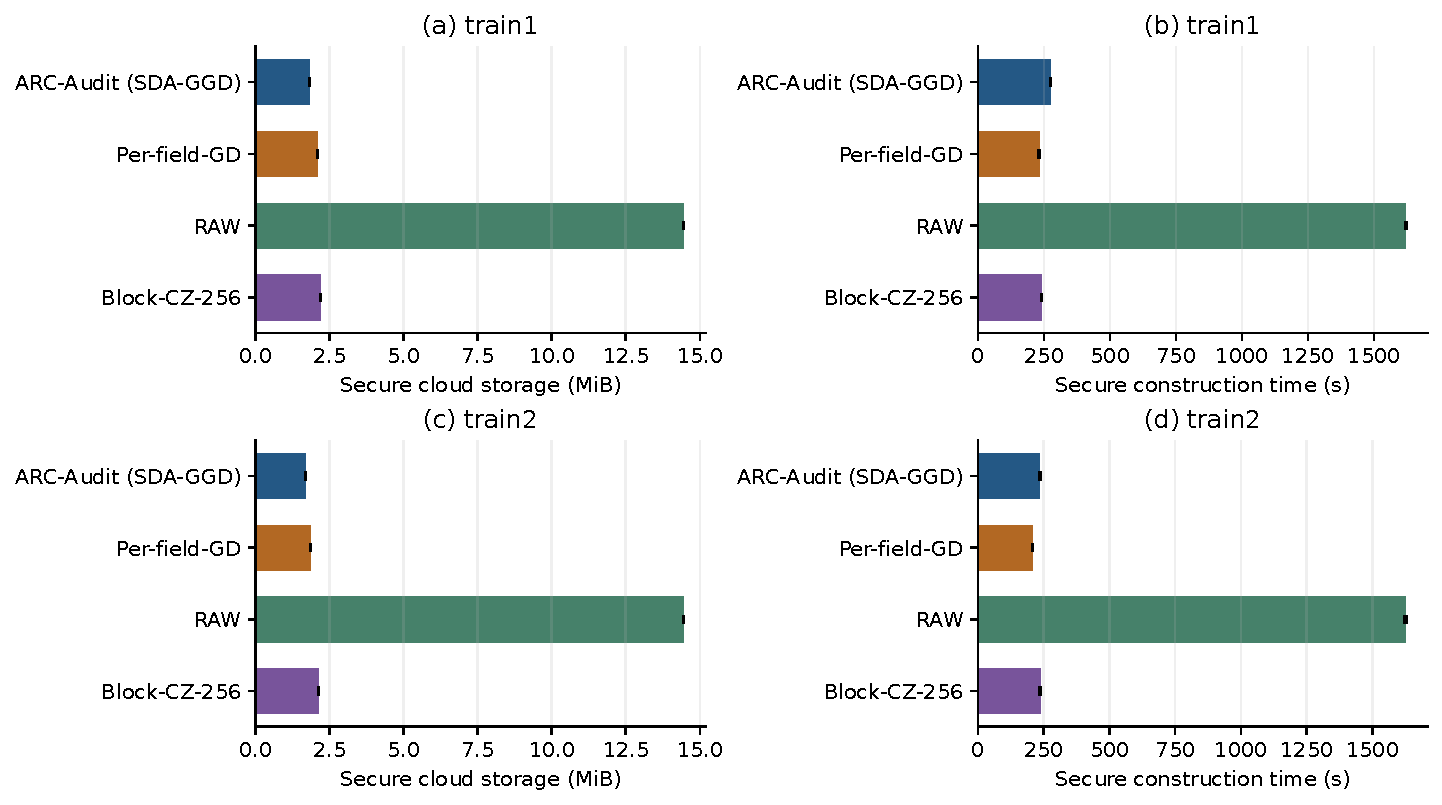
\includegraphics[width=\textwidth]{figures/c1_arc_audit.pdf}
\caption{Storage and construction costs of ARC-Audit (SDA-GGD) and the encoding baselines (RQ1).}
\label{fig:key-c1}\end{figure*}
\begin{figure*}[t]\centering
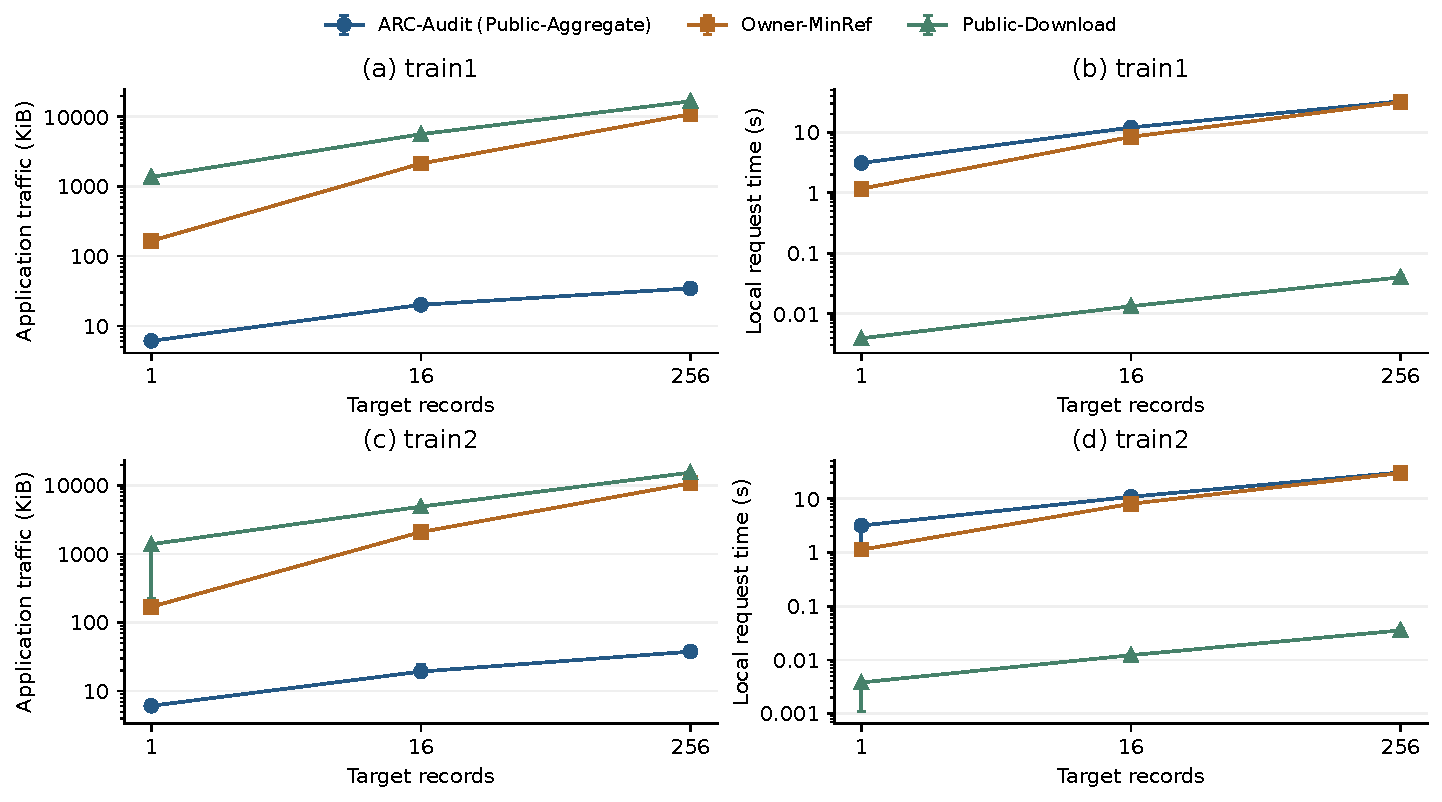
\includegraphics[width=\textwidth]{figures/c2_arc_audit.pdf}
\caption{Application traffic per request and local processing time with reused contexts (RQ2). Application traffic includes declarations, challenges, any first-stage material, and the final response. The break-even link rates reported in the text use a simple serial-transfer estimate.}
\label{fig:key-c2}\end{figure*}
\begin{figure*}[t]\centering
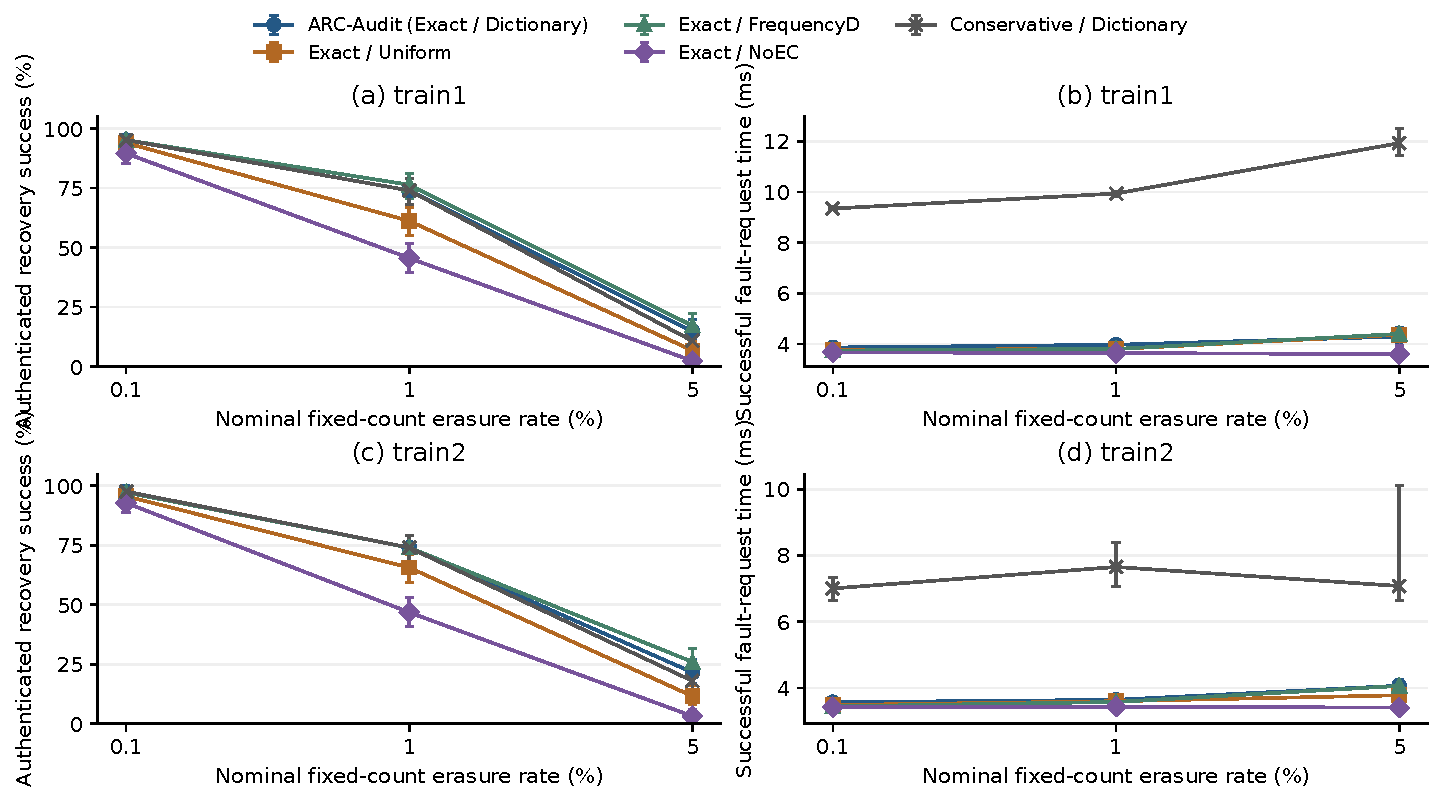
\includegraphics[width=\textwidth]{figures/c3_arc_audit.pdf}
\caption{Authenticated recovery under erasures (RQ3). ARC-Audit (Exact / Dictionary) combines exact recovery with dictionary-first protection.}
\label{fig:key-c3}\end{figure*}

\subsection{Experimental Setup}
\subsubsection{Data and Implementation}
We evaluate ARC-Audit on the \texttt{train1} and \texttt{train2} segments of the HAI 21.03 industrial control dataset~\cite{Shin2021HAI}, which contain 216,001 and 226,801 records, respectively. Each record comprises 84 columns: a timestamp, 79 process fields, and four attack indicators (three process-specific indicators encoded independently and one derived combined indicator). Exact decimal canonicalization during ingestion preserves process values. After each recovery operation, an independent scorer checks $\widehat r_i=r_i$ against the canonical source, separate from the client's authentication and complete-decoding checks.

The RQ1 encoding evaluation measures both six-hour windows of 21,600 records each (starting at 00:00 on July 11, 2020, for \texttt{train1} and August 1, 2020, for \texttt{train2}) and all seven full daily batches across both segments. The RQ2 auditing and RQ3 recovery evaluations likewise use all records. The three daily \texttt{train1} batches contain 86,400, 86,400, and 43,201 records, while the four daily \texttt{train2} batches contain 7,200, 86,400, 86,400, and 46,801 records. Each batch is configured and sealed independently. Because both segments come from a single HAI deployment, paired numeric results throughout this section follow \texttt{train1} and \texttt{train2} order.

The prototype is implemented in Python 3.10.12 using NumPy 2.2.6, cryptography 50.0.1, and py-ecc 8.0.0. It combines AES-256-GCM, Ed25519, the BLS12-381 full-page authenticator, and ciphertext RS$(10,8)$. Six-hour encoding measurements are pinned to CPU index 2 and full-workload measurements (full-batch encoding, RQ2 auditing, RQ2 representation controls, and RQ3 recovery) to CPU index 4 on the same host. Input preparation and independent scoring are excluded from the reported construction and request timings. Request timing begins at dependency planning inside an initialized, reusable batch context, and sidecar initialization also precedes the recovery timer.

\begin{table}[t]\centering\small
\caption{EVALUATION WORKLOADS}\label{tab:scope}
\setlength{\tabcolsep}{3.5pt}
\begin{tabular}{@{}l>{\raggedright\arraybackslash}p{.24\columnwidth}>{\raggedright\arraybackslash}p{.43\columnwidth}@{}}\toprule
Scope & Records per segment & Comparisons and observations\\\midrule
RQ1 (Windows) & 21,600 / 21,600 & 4 methods, 2 builds each (16 observations)\\
RQ1 (Full days) & 216,001 / 226,801 & 7 daily batches, 4 methods, 2 builds (56 observations)\\
RQ2 (Interfaces) & 216,001 / 226,801 & 3 target sizes, 3 cases, 3 interfaces (54 requests)\\
RQ2 (Rep. audit) & 216,001 / 226,801 & 3 target sizes, 3 cases, 2 codecs (36 matched requests)\\
RQ3 (Recovery) & 216,001 / 226,801 & 5 layouts, 3 loss rates, 50 cases, 8 controls (12,000 outcomes)\\
RQ3 (Budget $\beta$) & 216,001 / 226,801 & 4 budgets, 5 layouts, 2 loss rates, 4 controls (16,000 outcomes)\\
RQ3 (Clean) & Same as RQ3 & 30 cases, 1 layout, 8 controls (480 outcomes)\\
Active attacks & Daily snapshots & 6 attack classes, 20 trials each (120 trials)\\\bottomrule
\end{tabular}\end{table}

\subsubsection{Controls and Metrics}
For RQ1, we compare ARC-Audit's SDA-GGD encoder against Per-field-GD, RAW canonical encoding, and Block-CZ-256. Block-CZ-256 serializes nonconstant columns within blocks of 256 records and compresses each block as an independent Zstd frame at level 3. Per-field-GD applies GD independently to each nonconstant field to isolate the effect of cross-field grouping, while RAW and Block-CZ-256 serve as uncompressed and standard-compression baselines. All four representations share the same secure sealing and accounting rules. Secure cloud bytes include ciphertext, audit tags, and the signed public manifest, whereas owner base bytes and total private disk state are reported separately. Construction time covers configuration, encoding, and full secure sealing from normalized input.

The merge-ranking sample uses $\min(50{,}000,n)$ rows and therefore covers the full 21,600-row RQ1 window. This setting evaluates grouping with full-window ranking and full-input cost confirmation. We set $\rho=1$ so every tested prefix is feasible. Each method and window is built twice using seeds 41001 and 41002, and plots report the median and observed range.

For RQ2, we separate dependency discovery from proof response format across target counts $r\in\{1,16,256\}$, using three target sets per segment and target count. ARC-Audit's Public-Aggregate interface selects the public closure. Owner-MinRef-Aggregate (abbreviated as Owner-MinRef hereafter and in plots and tables) authenticates and decrypts the reference material needed to resolve exact dependencies, while Public-Download returns public-closure ciphertexts for hash verification. Neither public interface holds the decryption key, whereas Owner-MinRef holds authorized decryption capability. Comparing Public-Aggregate with Public-Download isolates response format under identical public access, whereas comparing Public-Aggregate with Owner-MinRef contrasts dependency planning across access capabilities.

Within each test case, all three interfaces evaluate the same targets, and cross-batch targets are served through their respective batch contexts. Application traffic includes declarations, challenges, first-stage reference material, and responses. Local request time covers dependency planning and interface execution, with initialization reported separately, so the time axis reflects local computation rather than network transfer. Each plotted point reports the median and min--max range across the three matched target sets.

For RQ3, we evaluate ARC-Audit under the Exact and Conservative dependency-selection policies across four protection configurations: Dictionary, Uniform, FrequencyD, and NoEC. Holding Exact fixed isolates protection placement, whereas holding a protection layout fixed isolates dependency selection, with NoEC serving as the zero-redundancy baseline.

All protected configurations share RS$(10,8)$, a common admitted stripe count, and a per-batch 10\% ciphertext-byte cap covering parity shards and signed sidecar metadata. FrequencyD ranks objects using the first $\min(4{,}096,\max(1,\lfloor n/5\rfloor))$ reference records of each batch, and all RQ3 recovery targets are drawn outside these reference ranges. Accordingly, the 7,200-record batch uses 1,440 reference records, and the remaining six batches each use 4,096. The independent scorer accesses source records only after the service timer stops, while recovery obtains inputs solely through the cloud fetch interface and verified repairs.

\subsubsection{Faults and Statistics}
For each segment, RQ3 evaluates five protection layouts generated with seeds 41001--41005 at nominal loss fractions $\alpha\in\{0.001,0.01,0.05\}$, using 50 single-record recovery cases per layout and loss rate. Each case selects one target record and draws a fixed-count erasure mask without replacement from the segment-wide union of original objects and deployed parity slots. The fault population sizes are $N_{\mathrm{fault}}=5{,}000$ on \texttt{train1} and $4{,}765$ on \texttt{train2}, yielding $\lceil\alpha N_{\mathrm{fault}}\rceil$ erasure counts of 5, 50, and 250 on \texttt{train1}, and 5, 48, and 239 on \texttt{train2}. Each target accesses only its own batch within this population. All controls share the same targets and slot-loss masks, with NoEC observing the corresponding original-page losses, and policy execution order is rotated across cases.

Each fault-success point aggregates all 250 outcomes with a pointwise 95\% Wilson confidence interval conditional on the five tested layouts. Recovery-time medians are computed over successful fault requests. Because different controls can succeed on different target subsets, recovery times should be interpreted alongside success probabilities. Clean recovery evaluates 30 cases per segment and control on a single layout, yielding 480 successful complete-record checks.



\subsection{RQ1: Storage and Secure Construction}
Cross-field grouping shrinks secure cloud storage relative to all baselines, though it shifts part of the encoding work to the owner. As shown in Fig.~\ref{fig:key-c1}, ARC-Audit (SDA-GGD) stores 1,903,138 B on \texttt{train1} and 1,770,118 B on \texttt{train2}, compared with 2,198,812 B and 1,938,839 B for Per-field-GD, corresponding to cloud storage reductions of 13.45\% and 8.70\%. Block-CZ-256 stores 2,278,001 B and 2,227,359 B, whereas RAW occupies 14.463 MiB per window. All 16 constructions pass canonical decoding checks.

Grouping increases total construction time because candidate merges are reconfigured against the full input, even though fewer output pages reduce subsequent tag generation. On the six-hour windows, median complete secure construction time rises from 231.521 s and 206.163 s under Per-field-GD to 274.356 s and 235.621 s under SDA-GGD, an increase of 18.50\% on \texttt{train1} and 14.29\% on \texttt{train2}. Specifically, SDA-GGD spends 73.66 s and 47.63 s in the codec stage versus 1.00 s and 0.83 s for Per-field-GD, while tag-generation time drops from 230.25 s and 205.05 s to 200.42 s and 187.72 s.

Cloud storage savings are also accompanied by larger owner-side private state (Table~\ref{tab:state}). On the six-hour windows, SDA-GGD retains 335,884 B and 215,702 B of private state in total (including 303,595 B and 184,687 B of base content), compared with 245,064 B and 209,287 B for Per-field-GD (including 208,267 B and 174,552 B of bases).

\emph{Full multi-day scaling and sampled ranking.}
Table~\ref{tab:state} also summarizes all seven full daily batches (56 builds across 216,001 and 226,801 records), where the 86,400-row batches exercise $\min(50{,}000,n)$ sampled merge ranking before full-input confirmation. Across the complete multi-day segments, SDA-GGD reduces total secure cloud storage to 19.601 MiB on \texttt{train1} and 18.738 MiB on \texttt{train2}, saving 10.79\% and 11.44\% relative to Per-field-GD (21.973 and 21.159 MiB) and 13.90\% and 19.43\% relative to Block-CZ-256 (22.765 and 23.256 MiB). At full daily scale, storing fewer pages cuts tag-generation time from 2,583.1 s to 2,244.4 s on \texttt{train1} and from 2,594.9 s to 2,193.0 s on \texttt{train2}. That reduction offsets most of SDA-GGD's codec cost (533.5 s and 528.2 s), holding total construction overhead to 7.05\% and 4.38\% above Per-field-GD. On \texttt{train2}, SDA-GGD finishes the full build in 2,722.4 s, which is 4.07\% faster than Block-CZ-256 (2,837.9 s). All 56 full-batch builds pass canonical decoding checks.

\begin{table}[t]\centering\footnotesize
\caption{STORAGE, OWNER STATE, AND CONSTRUCTION TIME (RQ1)}\label{tab:state}
\setlength{\tabcolsep}{2.4pt}
\begin{tabular}{@{}lrrrrrr@{}}\toprule
& \multicolumn{2}{c}{Cloud (MiB)} & \multicolumn{2}{c}{Owner (KiB)} & \multicolumn{2}{c}{Build (s)}\\
\cmidrule(lr){2-3}\cmidrule(lr){4-5}\cmidrule(l){6-7}
Method & t1 & t2 & t1 & t2 & t1 & t2\\\midrule
\multicolumn{7}{@{}l}{\emph{(a) Six-hour windows (21,600 / 21,600 records; 16 builds)}}\\
SDA-GGD & 1.815 & 1.688 & 328.0 & 210.6 & 274.4 & 235.6\\
Per-field-GD & 2.097 & 1.849 & 239.3 & 204.4 & 231.5 & 206.2\\
Block-CZ-256 & 2.172 & 2.124 & 0.2 & 0.2 & 241.7 & 236.7\\
RAW & 14.463 & 14.463 & 0.2 & 0.2 & 1,620.5 & 1,625.5\\\midrule
\multicolumn{7}{@{}l}{\emph{(b) Full multi-day segments (216,001 / 226,801 records; 56 builds)}}\\
SDA-GGD & 19.601 & 18.738 & 3,206.7 & 2,723.4 & 2,778.9 & 2,722.4\\
Per-field-GD & 21.973 & 21.159 & 1,755.4 & 1,742.4 & 2,595.8 & 2,608.1\\
Block-CZ-256 & 22.765 & 23.256 & 0.7 & 0.9 & 2,751.9 & 2,837.9\\
RAW & 144.458 & 151.702 & 0.7 & 0.9 & 17,282.2 & 18,590.7\\
\bottomrule\end{tabular}
\tabnote{Sums of per-batch medians over two builds per batch (t1 = \texttt{train1}, t2 = \texttt{train2}). SDA-GGD is ARC-Audit's grouped encoder. Owner state includes the base catalog and private encoding/key files. Protection is accounted separately.}
\end{table}

\subsection{RQ2: Public Audit Communication and Computation}
\emph{Aggregate proofs and ciphertext downloads.}
Over the same public closure, proof aggregation cuts application-layer traffic by more than two orders of magnitude at the cost of local cryptographic verification (Fig.~\ref{fig:key-c2}). At $r=256$, Public-Aggregate transfers 35,405 B on \texttt{train1} and 38,524 B on \texttt{train2} with local processing times of 32.532 s and 30.908 s. By contrast, Public-Download transfers 17,041,940 B and 15,754,868 B and verifies digests locally in 0.0400 s and 0.0354 s. Dividing the saved bits by the additional local processing time yields simple serial-transfer break-even link rates of 4.19 Mbit/s and 4.07 Mbit/s, excluding initialization, network round trips, and transfer--computation overlap.

\emph{Public planning and authorized reference discovery.}
Public closure planning eliminates first-stage reference transfer while matching the local runtime of authorized reference discovery at larger target sets. Owner-MinRef uses authenticated decryption of references to narrow its final dictionary coverage, which adds reference traffic. At $r=256$, Owner-MinRef transfers 11,163,473 B and 11,010,612 B with local processing times of 31.532 s and 30.148 s. Relative to Owner-MinRef, Public-Aggregate reduces application traffic by 99.68\% and 99.65\% (computed from observed medians) while increasing local processing by 3.17\% and 2.52\%.

At smaller target sets, reference discovery saves more local pairing work because each record touches fewer objects, though it still incurs substantial reference traffic. For $r=1$, Public-Aggregate transfers 6,237 B and 6,254 B in 3.106 s and 3.169 s locally, whereas Owner-MinRef transfers 169,601 B and 173,696 B in 1.164 s and 1.126 s. As $r$ grows, cross-target overlap and the union of references narrow this runtime gap: at $r=16$, Public-Aggregate transfers 20,512 B and 19,742 B in 12.015 s and 10.902 s, compared with 2,179,425 B and 2,138,835 B in 8.404 s and 8.066 s for Owner-MinRef.

\emph{Traffic composition and context reuse.}
Reference material dominates Owner-MinRef traffic at $r=256$, accounting for median first-stage transfers of 11,128,596 B and 10,972,500 B that both public interfaces avoid. Both aggregate interfaces return a 4,310 B proof per batch (12,930 B across the three \texttt{train1} batches and 17,240 B across the four \texttt{train2} batches), with declarations and challenges forming the remainder. The request timings above use initialized batch contexts reused across requests. Cold context setup requires a median of 8.101 s and 7.805 s at $r=1$, and fetches 1,678,681 B and 1,623,188 B of manifests and public parameters in 20.816 s and 21.168 s at $r=256$. All 54 honest requests pass verification under their respective interfaces.

\emph{Mechanism controls and full-workload representation audit.}
Table~\ref{tab:c2-mechanisms} isolates read reuse and proof aggregation on two single-batch 16-target requests from the July 11 \texttt{train1} batch and July 31 \texttt{train2} batch. Union planning and cached per-record traversal both read each selected object once, and aggregation sharply reduces proof size and verification time when pages and challenge coefficients are held fixed.

To evaluate how data representation affects public aggregate auditing across target scales and multi-batch requests, Table~\ref{tab:c2-rep-full} compares SDA-GGD and Per-field-GD across all 18 matched RQ2 cohorts ($r\in\{1,16,256\}$, three cases per segment) under the same Public-Aggregate backend, union planner, and CPU pinning. Closure sizes cross over as $r$ increases because shared dictionary pages are amortized across targets. At $r=1$, cross-field grouping produces larger group dictionaries (Table~\ref{tab:state}), so covering complete dictionaries without decryption keys requires 42.86\% and 43.57\% more closure pages under SDA-GGD than under Per-field-GD, increasing local processing by 26.97\% and 29.21\%. Around $r=16$, the two representations nearly match ($+5.80\%$ pages on \texttt{train1}, and $-3.25\%$ pages with $-7.15\%$ local time on \texttt{train2}). At $r=256$, union planning amortizes dictionary pages across targets and SDA-GGD's shorter per-record reference and deviation streams dominate, cutting closure pages and server reads by 14.33\% on \texttt{train1} and 17.88\% on \texttt{train2} and lowering local verification time by 13.13\% and 17.49\% across all six matched cohorts (6/6 wins) while keeping the 4,310 B per-batch proof unchanged.

\begin{table}[t]\centering\small
\caption{AUDIT MECHANISM CONTROLS FOR TWO 16-TARGET REQUESTS (RQ2)}
\label{tab:c2-mechanisms}
\setlength{\tabcolsep}{3.2pt}
\begin{tabular}{@{}lrrrr@{}}\toprule
 & \multicolumn{2}{c}{train1} & \multicolumn{2}{c}{train2}\\
\cmidrule(lr){2-3}\cmidrule(l){4-5}
Traversal & Reads & Bytes & Reads & Bytes\\\midrule
Per-record & 5,643 & 23,113,728 & 892 & 3,651,221\\
Per-record, cached & 805 & 3,297,280 & 125 & 509,589\\
Union & 805 & 3,297,280 & 125 & 509,589\\\midrule
Proof format & Bytes & Verify (s) & Bytes & Verify (s)\\\midrule
Individual & 3,475,990 & 472.659 & 539,750 & 73.646\\
Aggregate & 4,310 & 3.477 & 4,310 & 1.074\\\bottomrule
\end{tabular}
\tabnote{Per-record traversal without caching counts repeated reads. Proof-format rows hold selected pages and challenge coefficients fixed.}
\end{table}

\begin{table}[t]\centering\small
\caption{FULL-WORKLOAD REPRESENTATION AUDIT COMPARISON (RQ2)}
\label{tab:c2-rep-full}
\setlength{\tabcolsep}{3.0pt}
\begin{tabular}{@{}llrrrrrr@{}}\toprule
& & \multicolumn{2}{c}{Closure pages} & & \multicolumn{2}{c}{Local time (s)} & \\
\cmidrule(lr){3-4}\cmidrule(lr){6-7}
Seg. & $r$ & PF-GD & SDA & $\Delta$Pg & PF-GD & SDA & $\Delta$Time\\\midrule
train1 & 1 & 238 & 340 & +42.9\% & 2.651 & 3.355 & +27.0\%\\
 & 16 & 1,323 & 1,398 & +5.8\% & 13.369 & 13.521 & +2.2\%\\
 & 256 & 4,854 & 4,143 & \textbf{-14.3\%} & 39.944 & 34.767 & \textbf{-13.1\%}\\\midrule
train2 & 1 & 240 & 345 & +43.6\% & 2.553 & 3.298 & +29.2\%\\
 & 16 & 1,261 & 1,220 & \textbf{-3.3\%} & 13.127 & 12.502 & \textbf{-7.2\%}\\
 & 256 & 4,684 & 3,830 & \textbf{-17.9\%} & 39.207 & 32.705 & \textbf{-17.5\%}\\\bottomrule
\end{tabular}
\tabnote{Medians across all 18 matched multi-batch RQ2 cohorts (3 cases per row) under identical Public-Aggregate backend on CPU 4. PF-GD = Per-field-GD, SDA = SDA-GGD. Negative $\Delta$ indicates SDA-GGD savings (6/6 matched wins at $r=256$). Server read bytes scale proportionally to closure pages (e.g., at $r=256$: 19.88 vs.\ 16.97 MB on \texttt{train1}; 19.18 vs.\ 15.69 MB on \texttt{train2}).}
\end{table}

\subsection{RQ3: Authenticated Recovery and Protection Allocation}
\emph{Protection placement.}
Prioritizing dictionary pages consistently outperforms uniform redundancy under the same storage cap (Fig.~\ref{fig:key-c3}). With Exact recovery held fixed at 1\% nominal loss, Dictionary recovers 185 of 250 records (74.0\%) on both segments, whereas Uniform recovers 153 of 250 (61.2\%) on \texttt{train1} and 164 of 250 (65.6\%) on \texttt{train2}, representing gains of 12.8 and 8.4 percentage points, and NoEC recovers 114 of 250 (45.6\%) and 117 of 250 (46.8\%). At 0.1\% loss, Dictionary reaches 95.2\% and 97.6\%, compared with 94.0\% and 95.6\% for Uniform.

\emph{Frequency-based allocation.}
Ranking pages by reference-workload dependency frequency (FrequencyD) provides a modest further advantage over object-type ranking (Dictionary) at 5\% nominal loss. Under Exact recovery at 5\% loss, FrequencyD recovers 43 of 250 records (17.2\%) on \texttt{train1} and 65 of 250 (26.0\%) on \texttt{train2}, compared with 14.8\% and 21.6\% for Dictionary. Across the five tested layouts, paired differences range from $-2$ to $+8$ percentage points on \texttt{train1} and from $0$ to $+12$ percentage points on \texttt{train2} (Table~\ref{tab:paired-layouts}). With code, stripe count, and budget fixed, changing the ranking alters both which pages are protected and which pages share a stripe. At 1\% loss, FrequencyD recovers 191 of 250 and 185 of 250 records versus 185 of 250 on both segments for Dictionary, while at 0.1\% loss the two policies tie on \texttt{train1} and Dictionary is slightly ahead on \texttt{train2}.

\emph{Dependency policy.}
Under fixed Dictionary protection at 5\% nominal erasure, narrowing retrieval to exact dependencies enables recovery on requests where unused dictionary pages are lost. Exact recovers every record recovered by Conservative plus ten additional records on \texttt{train1} and nine on \texttt{train2}, raising complete-record recovery from 27 of 250 (10.8\%) to 37 of 250 (14.8\%) on \texttt{train1} and from 45 of 250 (18.0\%) to 54 of 250 (21.6\%) on \texttt{train2}. These improvements of 4.0 and 3.6 percentage points leave failure rates of 85.2\% and 78.4\% for Exact under the 10\% redundancy cap at 5\% erasure. In every additional successful case, all actual dependencies were retrievable or repairable while unreferenced dictionary pages were unavailable. At 0.1\% and 1\% nominal erasure, both policies succeed on the same requests.

\begin{table}[t]
\centering\small
\caption{PAIRED RECOVERY OUTCOMES AT 5\% LOSS (RQ3)}
\label{tab:paired-layouts}
\setlength{\tabcolsep}{3pt}
\begin{tabular}{@{}llrrrrr@{}}
\toprule
Segment & Pair & 41001 & 41002 & 41003 & 41004 & 41005 \\
\midrule
train1 & F/D & 0/1 & 2/2 & 5/1 & 3/1 & 4/3 \\
       & D/U & 9/0 & 3/1 & 3/3 & 2/0 & 8/1 \\
       & E/C & 3/0 & 1/0 & 1/0 & 2/0 & 3/0 \\
\midrule
train2 & F/D & 2/1 & 4/0 & 7/1 & 2/2 & 2/2 \\
       & D/U & 4/0 & 7/0 & 4/2 & 8/2 & 7/1 \\
       & E/C & 1/0 & 2/0 & 2/0 & 2/0 & 2/0 \\
\bottomrule
\end{tabular}
\tabnote{Columns are layout seeds. Each cell gives the cases recovered only by the first/second configuration out of 50 matched cases. F, D, and U are FrequencyD, Dictionary, and Uniform with Exact. E/C compares Exact and Conservative with Dictionary fixed.}
\end{table}

\emph{Recovery time.}
Exact recovery also reduces latency because it fetches and decrypts fewer authenticated bytes. In clean Dictionary runs, where both policies recover the same targets, Exact completes in 3.693 ms on \texttt{train1} and 3.507 ms on \texttt{train2}, compared with 8.991 ms and 7.205 ms for Conservative. At 5\% nominal loss under Dictionary protection, successful requests take a median of 4.298 ms and 4.074 ms with Exact versus 11.933 ms and 7.079 ms with Conservative (including retrieval and any required RS repair), while failed requests terminate in medians of 0.414 ms and 0.461 ms for Exact versus 5.810 ms and 3.892 ms for Conservative. Because the two policies succeed on different request sets under faults, successful-request medians reflect completion times within each policy's own successful subset.

Taken together, protection allocation determines which objects receive redundancy and dependency selection determines which objects a request requires. Reducing the required page set under fixed protection and verification rules therefore enables more requests to complete within the tested HAI workloads and erasure settings.

\emph{Protection budget sensitivity.}
To evaluate how recoverability scales beyond the $\beta=0.10$ cap, Table~\ref{tab:budget-sweep} sweeps $\beta\in\{0.10,0.15,0.20,0.30\}$ over the same five layouts and 250 matched cases per segment at $\alpha\in\{0.01,0.05\}$. Because systematic RS$(10,8)$ requires $\approx 25\%$ parity overhead plus sidecar metadata, raising $\beta$ from 0.10 to 0.30 expands protected page coverage from 38.8\%/38.7\% to 100.0\%. At 1\% nominal erasure, complete-record recovery under Exact/Dictionary climbs from 74.0\% on both segments to 100.0\% on \texttt{train1} and 99.6\% on \texttt{train2} (with Exact/FrequencyD reaching 100.0\% on both). Under 5\% erasure, Exact/Dictionary rises from 14.8\% to 72.4\% on \texttt{train1} and from 21.6\% to 76.4\% on \texttt{train2} (Exact/FrequencyD reaches 76.8\% and 80.0\%). Once $\beta=0.30$ covers all pages, placement differences between Dictionary and Uniform largely disappear (72.4\% vs.\ 75.6\% on \texttt{train1}, and 76.4\% vs.\ 74.4\% on \texttt{train2}). By contrast, the advantage of Exact over Conservative widens from $+4.0$ and $+3.6$ percentage points at $\beta=0.10$ to $+20.0$ and $+12.4$ percentage points at $\beta=0.30$ (72.4\% vs.\ 52.4\% and 76.4\% vs.\ 64.0\%), because Conservative still fails whenever any unreferenced dictionary stripe suffers three or more erasures.

\begin{table}[t]\centering\small
\caption{RECOVERY RATE ACROSS PROTECTION BUDGETS $\beta$ (RQ3)}
\label{tab:budget-sweep}
\setlength{\tabcolsep}{3.0pt}
\begin{tabular}{@{}lcrrrrrrr@{}}\toprule
& & & \multicolumn{3}{c}{$\alpha=0.01$ (\%)} & \multicolumn{3}{c}{$\alpha=0.05$ (\%)}\\
\cmidrule(lr){4-6}\cmidrule(l){7-9}
Seg. & $\beta$ & Cov. & E/D & E/U & E/F & E/D & C/D & E/F\\\midrule
train1 & 0.10 & 38.8\% & 74.0 & 61.2 & 76.4 & 14.8 & 10.8 & 17.2\\
 & 0.15 & 58.3\% & 76.0 & 72.0 & 78.8 & 22.0 & 18.8 & 29.6\\
 & 0.20 & 77.8\% & 86.8 & 79.6 & 88.4 & 34.0 & 24.8 & 41.6\\
 & 0.30 & 100.0\% & 100.0 & 100.0 & 100.0 & 72.4 & 52.4 & 76.8\\\midrule
train2 & 0.10 & 38.7\% & 74.0 & 65.6 & 74.0 & 21.6 & 18.0 & 26.0\\
 & 0.15 & 58.2\% & 77.2 & 70.8 & 80.0 & 28.0 & 26.4 & 36.0\\
 & 0.20 & 77.9\% & 84.0 & 82.4 & 86.4 & 45.2 & 37.6 & 49.2\\
 & 0.30 & 100.0\% & 99.6 & 100.0 & 100.0 & 76.4 & 64.0 & 80.0\\\bottomrule
\end{tabular}
\tabnote{Each cell aggregates 250 matched outcomes (5 layouts $\times$ 50 cases). Cov.\ is the protected ciphertext-page fraction. E/D, E/U, E/F denote Exact with Dictionary, Uniform, and FrequencyD; C/D denotes Conservative with Dictionary (at $\alpha=0.01$, C/D matches E/D within 0.4 percentage points across all budgets; at $\alpha=0.05$ and $\beta=0.30$, E/U is 75.6\% on \texttt{train1} and 74.4\% on \texttt{train2}).}
\end{table}

\subsection{Active Adversary Verification}\label{sec:attacks}
To validate our security analysis empirically against an active malicious CSP, we executed 120 adversarial trials spanning six attack classes on sealed daily snapshots from both HAI segments (\texttt{train1\_2020-07-11} and \texttt{train2\_2020-08-01}, 10 deterministic trials per class per segment). Table~\ref{tab:attacks} summarizes the tested attacks and detection outcomes. Every attack across all six classes is rejected (120/120), confirming that ciphertext or tag forgery fails aggregate pairing verification (Eq.~\eqref{eq:pairing}), replaying an honest proof from a prior challenge fails fresh nonce/context binding, single-bit manifest tampering fails client pin and Ed25519 verification, corrupted parity shards are rejected prior to RS decoding without outputting unauthenticated records, and cross-snapshot RS sidecars are blocked by snapshot-digest binding.

\begin{table}[t]\centering\small
\caption{ACTIVE ADVERSARY VERIFICATION MATRIX}
\label{tab:attacks}
\setlength{\tabcolsep}{3.0pt}
\begin{tabular}{@{}l>{\raggedright\arraybackslash}p{.40\columnwidth}c@{}}\toprule
Attack Class & Enforcing Mechanism & Rejected\\\midrule
Ciphertext tampering (audit) & Pairing check (Eq.~\eqref{eq:pairing}) & 20/20\\
Audit tag substitution & Descriptor hash $H(W_p)$ \& pairing & 20/20\\
Stale-challenge proof replay & Fresh nonce \& challenge binding & 20/20\\
Manifest / layout tampering & Client digest pin \& Ed25519 sig. & 20/20\\
Corrupted RS parity repair & Parity SHA-256 \& AEAD verify & 20/20\\
Cross-snapshot sidecar swap & Sidecar snapshot-digest binding & 20/20\\\bottomrule
\end{tabular}
\tabnote{10 deterministic trials per segment (\texttt{train1} and \texttt{train2}) per attack class; zero false accepts or unauthenticated record outputs observed.}
\end{table}

\subsection{Experimental Artifacts}
All six-hour and full-workload encoding runs (RQ1), full-workload auditing and recovery runs (RQ2 and RQ3), case-level observations, mechanism controls, source snapshots, and hash-verified configuration manifests are preserved in the archived evaluation bundle (\texttt{dual\_hai\_20261008\_v3}). Automated verification scripts recompute all reported summary statistics and validate serialized per-batch protection caps against the archived manifests.

\subsection{Discussion and Practical Deployment}\label{sec:discussion}
\emph{Cryptographic backend versus protocol overhead.}
In RQ2, local verification for 256 targets takes 32.532 s on \texttt{train1} and 30.908 s on \texttt{train2}, while tag generation in RQ1 accounts for 187.7--200.4 s per six-hour window (2,193.0--2,244.4 s across full multi-day segments). These runtimes come from our pure-Python \texttt{py-ecc} reference implementation, chosen to keep the prototype self-contained and bit-level reproducible. To separate protocol cost from Python interpreter overhead, we benchmarked the identical multi-batch Eq.~\eqref{eq:aggregate}--\eqref{eq:pairing} prover and verifier workload ($s=133$, matched closure page counts, single-core CPU~4 pinning) using the assembly-accelerated Rust \texttt{blst} (v0.3.17) BLS12-381 library with Pippenger multi-scalar multiplication. At $r=256$, total prover-plus-verifier time drops from 34.77 s (\texttt{train1}) and 32.71 s (\texttt{train2}) under \texttt{py-ecc} to 100.81 ms and 100.79 ms with cached descriptor hashes (a 324.5$\times$--344.9$\times$ speedup, with 45.4--45.6 ms verifier-only), and to 252.4--266.7 ms even when recomputing hash-to-curve cold per request. This native backend raises the simple serial break-even link rate at $r=256$ from 4.07--4.19 Mbit/s to above 1.2 Gbit/s, while the fixed 4,310 B per-batch proof size stays independent of implementation language.

\emph{Interpreting erasure regimes and protection budgets.}
At 0.1\% and 1\% nominal object loss, dictionary-first RS$(10,8)$ under a 10\% storage cap recovers 95.2\%--97.6\% and 74.0\% of requested records, and raising $\beta$ to 0.30 reaches 99.6\%--100.0\% recovery at 1\% loss. At 5\% nominal loss, unreferenced dictionary pages frequently fail, exposing the 12.4--20.0 percentage-point advantage of exact dependency resolution ($D(T)$) over conservative closure retrieval ($U(T)$) once full-batch RS protection is provisioned ($\beta=0.30$).

\emph{Scope boundaries and operational trade-offs.}
Our evaluation covers seven daily batches, 18 matched multi-batch audit cohorts, and four redundancy budgets from two segments of one industrial control testbed (HAI 21.03), so compression ratios and dependency skew on other IIoT schemas remain to be measured. In addition, ARC-Audit seals immutable daily batches independently to keep snapshot pinning and keys batch-local rather than supporting in-place record updates or cross-batch dictionary reuse. Supporting dynamic appends or shared multi-batch dictionaries would require versioned manifest chains and incremental dictionary indexing, as in dynamic block-auditing schemes~\cite{Pan2026,Xu2026MPA}. Client metadata also scales with the batch page count $N$ (1.62--1.68 MB across the multi-day HAI segments). Archival servers and IIoT gateways can cache these manifests directly, whereas memory-constrained edge verifiers can fetch authenticated manifest slices on demand using Merkle commitments.

\section{Conclusion}
ARC-Audit uses a single authenticated layout to reconcile public auditing and authorized recovery over shared-compressed IIoT records. Without decryption keys, a public verifier builds a sufficient closure covering all dictionary pages a target set could reference and binds it to a fresh aggregate challenge. With decryption keys, an authorized retriever authenticates references first to narrow retrieval to exact dependencies, while verifying repaired and directly fetched ciphertexts under identical integrity rules.

Across two multi-day HAI segments, ARC-Audit's grouped representation reduced secure cloud storage by 10.79\% and 11.44\% relative to per-field GD (13.45\% and 8.70\% on six-hour windows) while adding only 4.38\%--7.05\% full-batch construction overhead. Over the same public closure, aggregate auditing cut application traffic by more than two orders of magnitude. Across 18 matched multi-batch cohorts, grouped dictionaries enlarged single-record closures ($r=1$) yet reduced closure pages by 14.33\%--17.88\% and local verification time by 13.13\%--17.49\% at $r=256$. All 120 active-adversary trials spanning six attack classes were rejected. Under erasures, dictionary-first RS$(10,8)$ at a 10\% budget recovered 95.2\%--97.6\% of records at 0.1\% loss and 74.0\% at 1\% loss. Raising the budget to 30\% lifted recovery to 99.6\%--100.0\% at 1\% loss and 72.4\%--76.4\% at 5\% loss, widening exact-versus-conservative recovery gains from 3.6--4.0 to 12.4--20.0 percentage points. Future work will extend the authenticated dependency map to cross-batch shared dictionaries, quantify index and manifest update costs, evaluate repair read amplification under correlated and whole-batch failures, and validate these policies across additional IIoT datasets.

\bibliographystyle{IEEEtran}
\bibliography{IEEEabrv,bstcontrol,references}
\end{document}

